\documentclass[aspectratio=169, 11pt]{beamer}

% ── Theme matching the t-SNE reference lecture ──
\usetheme{Madrid}
\usecolortheme{whale}
\setbeamercolor{frametitle}{bg=blue!8, fg=black}
\setbeamercolor{title}{bg=blue!12, fg=black}
\setbeamercolor{structure}{fg=blue!50!black}
\setbeamercolor{item}{fg=blue!50!black}
\setbeamertemplate{navigation symbols}{}
\setbeamertemplate{footline}{
  \leavevmode\hbox{%
    \begin{beamercolorbox}[wd=.35\paperwidth,ht=2.5ex,dp=1ex,left]{author in head/foot}%
      \hspace*{1em}\footnotesize Machine Learning with R (Dr.\ Endri Ra\c{c}o)
    \end{beamercolorbox}%
    \begin{beamercolorbox}[wd=.35\paperwidth,ht=2.5ex,dp=1ex,center]{title in head/foot}%
      \footnotesize Statistical Learning \& Linear Regression
    \end{beamercolorbox}%
    \begin{beamercolorbox}[wd=.3\paperwidth,ht=2.5ex,dp=1ex,right]{date in head/foot}%
      \footnotesize Week 1, 2025 \hspace*{1em} \insertframenumber{} / \inserttotalframenumber \hspace*{1em}
    \end{beamercolorbox}}%
}

\usepackage{amsmath,amssymb,mathtools}
\usepackage{tikz}
\usetikzlibrary{arrows.meta, positioning, calc, shapes, decorations.pathreplacing, patterns}
\usepackage{pgfplots}
\pgfplotsset{compat=1.18}
\usepackage{booktabs}
\usepackage{xcolor}

\definecolor{accent}{RGB}{59,130,246}
\definecolor{darkblue}{RGB}{30,39,97}
\definecolor{softred}{RGB}{239,68,68}
\definecolor{softgreen}{RGB}{16,185,129}
\definecolor{amber}{RGB}{245,158,11}
\definecolor{muted}{RGB}{100,116,139}

\newcommand{\bhat}{\hat{\beta}}
\newcommand{\yhat}{\hat{y}}
\newcommand{\fhat}{\hat{f}}

\title{Statistical Learning \& Linear Regression}
\subtitle{A Visual Journey Through ISLR Chapters 2--3}
\author{Machine Learning with R}
\institute{Dr.\ Endri Ra\c{c}o}
\date{Week 1, 2025}

\begin{document}

% ══════════════════════════════════════════════
% TITLE
% ══════════════════════════════════════════════
\begin{frame}
\titlepage
\end{frame}

% ══════════════════════════════════════════════
% PART I: STATISTICAL LEARNING
% ══════════════════════════════════════════════

\begin{frame}{The Fundamental Problem}
\begin{columns}
\column{0.48\textwidth}
\textbf{Given:}
\begin{itemize}
  \item Data: $(x_1, y_1), \ldots, (x_n, y_n)$
  \item $x_i \in \mathbb{R}^p$ (predictors)
  \item $y_i \in \mathbb{R}$ (response)
\end{itemize}

\vspace{0.5em}
\textbf{Find:}
$$Y = f(X) + \varepsilon$$

\vspace{0.5em}
$f$ = \textcolor{accent}{systematic signal}\\
$\varepsilon$ = \textcolor{softred}{random noise}, $E[\varepsilon] = 0$

\column{0.48\textwidth}
\textbf{Key Question:}

\vspace{0.3em}
What is the \textbf{shape} of $f$?

\vspace{0.5em}
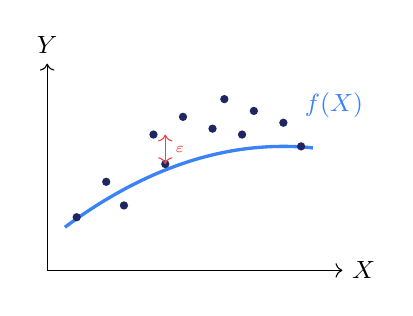
\begin{tikzpicture}[scale=0.75]
  \draw[->] (0,0) -- (5,0) node[right] {\small $X$};
  \draw[->] (0,0) -- (0,3.5) node[above] {\small $Y$};
  % True function
  \draw[accent, very thick, domain=0.3:4.5, samples=50] plot (\x, {0.5 + 0.8*\x - 0.1*\x*\x});
  % Data points with noise
  \foreach \x/\y in {0.5/0.9, 1/1.5, 1.3/1.1, 1.8/2.3, 2/1.8, 2.3/2.6, 2.8/2.4, 3/2.9, 3.3/2.3, 3.5/2.7, 4/2.5, 4.3/2.1} {
    \fill[darkblue] (\x, \y) circle (2pt);
  }
  \node[accent, right] at (4.2, 2.8) {\small $f(X)$};
  \draw[<->, softred] (2, 1.8) -- (2, 2.3) node[midway, right] {\tiny $\varepsilon$};
\end{tikzpicture}
\end{columns}
\end{frame}


\begin{frame}{A Real Example: Advertising Data}
\begin{columns}
\column{0.45\textwidth}
\textbf{200 markets observed:}
\begin{itemize}
  \item $Y$ = Sales (thousands)
  \item $X_1$ = TV budget (\$k)
  \item $X_2$ = Radio budget (\$k)
  \item $X_3$ = Newspaper budget (\$k)
\end{itemize}

\vspace{0.5em}
\textbf{The manager asks:}
\begin{enumerate}
  \item Does advertising work?
  \item Which media matter?
  \item How much should we spend?
\end{enumerate}

\column{0.5\textwidth}
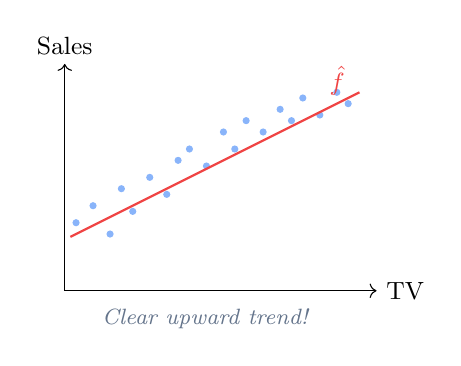
\begin{tikzpicture}[scale=0.72]
  \draw[->] (0,0) -- (5.5,0) node[right] {\small TV};
  \draw[->] (0,0) -- (0,4) node[above] {\small Sales};
  \foreach \x/\y in {0.2/1.2, 0.5/1.5, 0.8/1.0, 1.0/1.8, 1.2/1.4, 1.5/2.0, 1.8/1.7, 2.0/2.3, 2.2/2.5, 2.5/2.2, 2.8/2.8, 3.0/2.5, 3.2/3.0, 3.5/2.8, 3.8/3.2, 4.0/3.0, 4.2/3.4, 4.5/3.1, 4.8/3.5, 5.0/3.3} {
    \fill[accent!60] (\x, \y) circle (1.8pt);
  }
  \draw[softred, thick, domain=0.1:5.2, samples=30] plot (\x, {0.9 + 0.5*\x});
  \node[softred, right] at (4.5, 3.7) {\small $\hat{f}$};
  \node[muted] at (2.5, -0.5) {\footnotesize \textit{Clear upward trend!}};
\end{tikzpicture}
\end{columns}
\end{frame}


\begin{frame}{Why Estimate $f$? Two Goals}
\begin{columns}
\column{0.48\textwidth}
\textbf{\textcolor{accent}{Prediction}}

$$\hat{Y} = \hat{f}(X)$$

\begin{itemize}
  \item $f$ can be a \textbf{black box}
  \item We only care about $\hat{Y}$ accuracy
  \item Complex models OK
\end{itemize}

\vspace{0.5em}
\textit{Example:} Stock price tomorrow

\column{0.48\textwidth}
\textbf{\textcolor{softgreen}{Inference}}

$$Y = \beta_0 + \beta_1 X_1 + \cdots$$

\begin{itemize}
  \item We want to understand $f$ itself
  \item \textbf{Which} $X_j$ matter?
  \item \textbf{How} does each affect $Y$?
\end{itemize}

\vspace{0.5em}
\textit{Example:} Which ads drive sales?
\end{columns}

\vspace{1em}
\centering
\fbox{\parbox{0.6\textwidth}{\centering
Most real problems involve \textbf{both} goals\\
$\Rightarrow$ choose method accordingly}}
\end{frame}


\begin{frame}{Reducible vs.\ Irreducible Error}
\begin{columns}
\column{0.55\textwidth}
$$E\big[(Y - \hat{Y})^2\big] = \underbrace{[f(X) - \hat{f}(X)]^2}_{\text{reducible}} + \underbrace{\text{Var}(\varepsilon)}_{\text{irreducible}}$$

\vspace{0.8em}
\textbf{Reducible:} Better model $\Rightarrow$ smaller error

\textbf{Irreducible:} $\text{Var}(\varepsilon)$ is the floor

\vspace{0.5em}
No model can predict better than $\text{Var}(\varepsilon)$!

\column{0.4\textwidth}
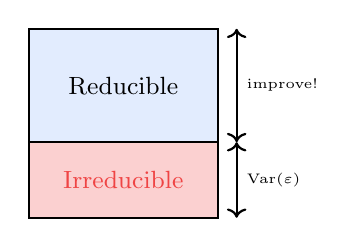
\begin{tikzpicture}[scale=0.8]
  \fill[accent!15] (0,0) rectangle (3,3);
  \fill[softred!25] (0,0) rectangle (3,1.2);
  \draw[thick] (0,0) rectangle (3,3);
  \draw[thick] (0,1.2) -- (3,1.2);
  \node at (1.5, 2.1) {\small Reducible};
  \node at (1.5, 0.6) {\small \textcolor{softred}{Irreducible}};
  \draw[<->, thick] (3.3, 0) -- (3.3, 1.2) node[midway, right] {\tiny $\text{Var}(\varepsilon)$};
  \draw[<->, thick] (3.3, 1.2) -- (3.3, 3) node[midway, right] {\tiny improve!};
\end{tikzpicture}
\end{columns}
\end{frame}


\begin{frame}{Parametric vs.\ Non-Parametric}
\begin{columns}
\column{0.48\textwidth}
\textbf{Parametric:}

Step 1: Assume a form
$$f(X) = \beta_0 + \beta_1 X_1 + \cdots + \beta_p X_p$$

Step 2: Fit (estimate $\beta$'s)

\vspace{0.3em}
\begin{itemize}
  \item[\textcolor{softgreen}{\textbullet}] Simple: estimate $p+1$ numbers
  \item[\textcolor{softred}{\textbullet}] May not match true $f$
\end{itemize}

\column{0.48\textwidth}
\textbf{Non-Parametric:}

No assumed form for $f$

\vspace{0.3em}
Get ``close'' to data without being too wiggly

\vspace{0.3em}
\begin{itemize}
  \item[\textcolor{softgreen}{\textbullet}] Flexible: many shapes
  \item[\textcolor{softred}{\textbullet}] Needs \textbf{lots} of data
  \item[\textcolor{softred}{\textbullet}] Overfitting risk
\end{itemize}
\end{columns}

\vspace{0.8em}
\centering
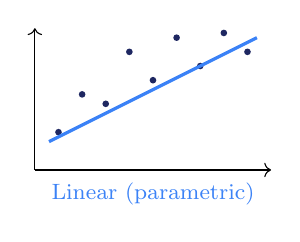
\begin{tikzpicture}[scale=0.6]
  \draw[->] (0,0) -- (5,0); \draw[->] (0,0) -- (0,3);
  \foreach \x/\y in {0.5/0.8, 1/1.6, 1.5/1.4, 2/2.5, 2.5/1.9, 3/2.8, 3.5/2.2, 4/2.9, 4.5/2.5} {
    \fill[darkblue] (\x,\y) circle (2pt);
  }
  \draw[accent, very thick] (0.3, 0.6) -- (4.7, 2.8);
  \node[accent] at (2.5, -0.5) {\footnotesize Linear (parametric)};
\end{tikzpicture}
\hspace{1cm}
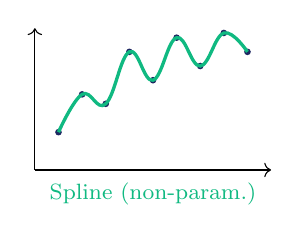
\begin{tikzpicture}[scale=0.6]
  \draw[->] (0,0) -- (5,0); \draw[->] (0,0) -- (0,3);
  \foreach \x/\y in {0.5/0.8, 1/1.6, 1.5/1.4, 2/2.5, 2.5/1.9, 3/2.8, 3.5/2.2, 4/2.9, 4.5/2.5} {
    \fill[darkblue] (\x,\y) circle (2pt);
  }
  \draw[softgreen, very thick, smooth, tension=0.7] plot coordinates {(0.5,0.8) (1,1.6) (1.5,1.4) (2,2.5) (2.5,1.9) (3,2.8) (3.5,2.2) (4,2.9) (4.5,2.5)};
  \node[softgreen] at (2.5, -0.5) {\footnotesize Spline (non-param.)};
\end{tikzpicture}
\end{frame}


\begin{frame}{The Flexibility--Interpretability Trade-Off}

\begin{center}
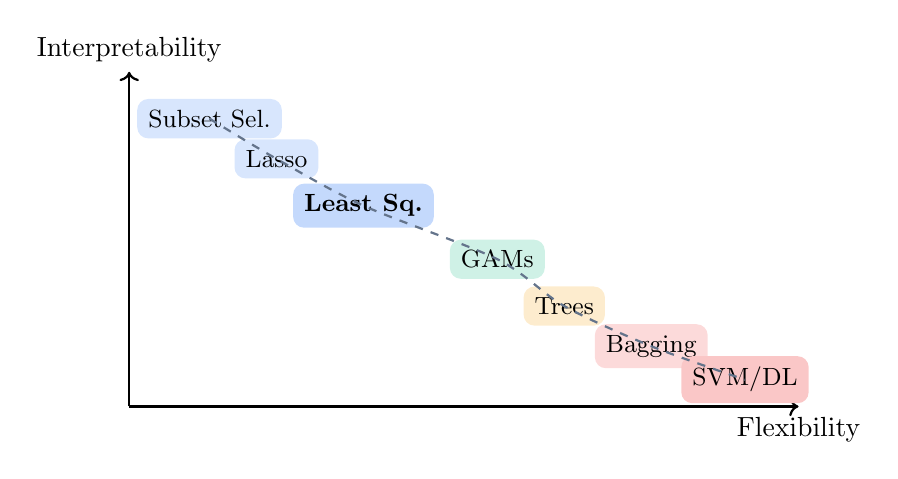
\begin{tikzpicture}[scale=0.85]
  % Axes
  \draw[->, thick] (0,0) -- (10,0) node[below] {Flexibility};
  \draw[->, thick] (0,0) -- (0,5) node[above] {Interpretability};

  % Methods
  \node[fill=accent!20, rounded corners, inner sep=4pt, font=\small] (ss) at (1.2, 4.3) {Subset Sel.};
  \node[fill=accent!20, rounded corners, inner sep=4pt, font=\small] (la) at (2.2, 3.7) {Lasso};
  \node[fill=accent!30, rounded corners, inner sep=4pt, font=\small\bfseries] (ls) at (3.5, 3.0) {Least Sq.};
  \node[fill=softgreen!20, rounded corners, inner sep=4pt, font=\small] (gam) at (5.5, 2.2) {GAMs};
  \node[fill=amber!20, rounded corners, inner sep=4pt, font=\small] (tr) at (6.5, 1.5) {Trees};
  \node[fill=softred!20, rounded corners, inner sep=4pt, font=\small] (bg) at (7.8, 0.9) {Bagging};
  \node[fill=softred!30, rounded corners, inner sep=4pt, font=\small] (sv) at (9.2, 0.4) {SVM/DL};

  % Dashed curve
  \draw[muted, thick, dashed, smooth, tension=0.5] plot coordinates {(1.2,4.3) (2.2,3.7) (3.5,3.0) (5.5,2.2) (6.5,1.5) (7.8,0.9) (9.2,0.4)};
\end{tikzpicture}
\end{center}

\vspace{-0.3em}
\centering
\textit{More flexible $\neq$ better predictions!}
\end{frame}


\begin{frame}{Measuring Fit: Mean Squared Error}
\begin{columns}
\column{0.5\textwidth}
$$\text{MSE} = \frac{1}{n}\sum_{i=1}^{n}\big(y_i - \hat{f}(x_i)\big)^2$$

\vspace{0.5em}
\textbf{Training MSE:} computed on data used to fit

\textbf{Test MSE:} computed on \textbf{new} data

\vspace{0.5em}
\textcolor{softred}{\textbf{We care about test MSE!}}

\column{0.45\textwidth}
\textbf{Numerical example:}

\vspace{0.3em}
\begin{tabular}{ccc}
\toprule
$y_i$ & $\hat{y}_i$ & $(y_i - \hat{y}_i)^2$ \\
\midrule
3.0 & 2.8 & 0.04 \\
5.0 & 4.5 & 0.25 \\
7.0 & 7.2 & 0.04 \\
4.0 & 4.8 & 0.64 \\
\bottomrule
\end{tabular}

\vspace{0.4em}
$\text{MSE} = \frac{0.04 + 0.25 + 0.04 + 0.64}{4} = 0.24$
\end{columns}
\end{frame}


\begin{frame}{Training MSE vs.\ Test MSE}

\begin{center}
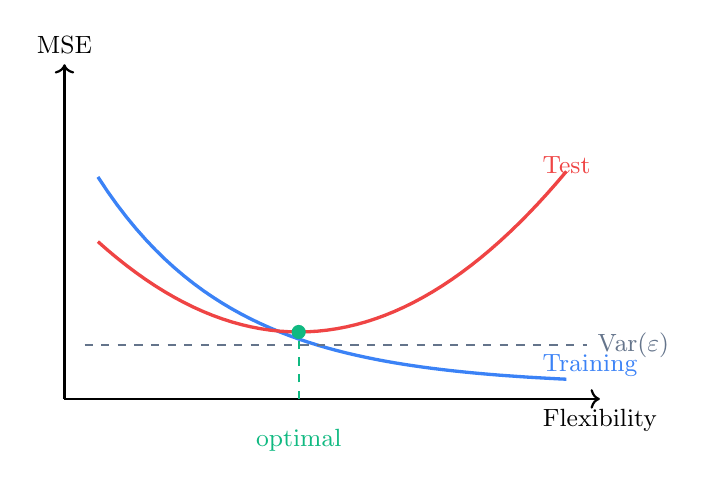
\begin{tikzpicture}[scale=0.85]
  \draw[->, thick] (0,0) -- (8,0) node[below] {\small Flexibility};
  \draw[->, thick] (0,0) -- (0,5) node[above] {\small MSE};

  % Training MSE - always decreasing
  \draw[accent, very thick, domain=0.5:7.5, samples=50] plot (\x, {4*exp(-0.5*\x) + 0.2});
  \node[accent, right] at (7, 0.5) {\small Training};

  % Test MSE - U-shaped
  \draw[softred, very thick, domain=0.5:7.5, samples=50] plot (\x, {0.15*(\x-3.5)*(\x-3.5) + 1.0});
  \node[softred, right] at (7, 3.5) {\small Test};

  % Irreducible error
  \draw[muted, dashed, thick] (0.3, 0.8) -- (7.8, 0.8);
  \node[muted] at (8.5, 0.8) {\small $\text{Var}(\varepsilon)$};

  % Optimal point
  \draw[softgreen, thick, dashed] (3.5, 0) -- (3.5, 1.0);
  \fill[softgreen] (3.5, 1.0) circle (3pt);
  \node[softgreen, below] at (3.5, -0.3) {\small optimal};
\end{tikzpicture}
\end{center}

\vspace{-0.3em}
\begin{itemize}
  \item Training MSE \textbf{always} decreases with flexibility
  \item Test MSE is \textbf{U-shaped} $\Rightarrow$ sweet spot exists
  \item Past the sweet spot: \textcolor{softred}{overfitting}
\end{itemize}
\end{frame}


\begin{frame}{The Bias-Variance Decomposition}

$$E\big[(y_0 - \hat{f}(x_0))^2\big] = \underbrace{\text{Var}(\hat{f}(x_0))}_{\text{variance}} + \underbrace{[\text{Bias}(\hat{f}(x_0))]^2}_{\text{bias}^2} + \underbrace{\text{Var}(\varepsilon)}_{\text{irreducible}}$$

\vspace{0.8em}
\begin{columns}
\column{0.48\textwidth}
\textbf{Bias} = systematic error

\vspace{0.2em}
Simple model $\Rightarrow$ high bias

\vspace{0.3em}
\textit{Example:} Fitting a line when truth is quadratic

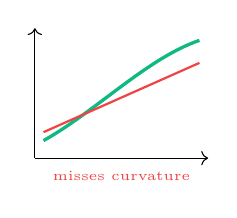
\begin{tikzpicture}[scale=0.55]
  \draw[->] (0,0) -- (4,0); \draw[->] (0,0) -- (0,3);
  \draw[softgreen, very thick, domain=0.2:3.8, samples=30] plot (\x, {0.3 + 0.5*\x + 0.15*\x*\x - 0.03*\x*\x*\x});
  \draw[softred, thick] (0.2, 0.6) -- (3.8, 2.2);
  \node[softred] at (2, -0.4) {\tiny misses curvature};
\end{tikzpicture}

\column{0.48\textwidth}
\textbf{Variance} = sensitivity to training data

\vspace{0.2em}
Complex model $\Rightarrow$ high variance

\vspace{0.3em}
\textit{Example:} Different datasets give wildly different curves

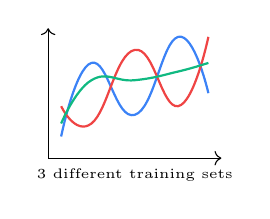
\begin{tikzpicture}[scale=0.55]
  \draw[->] (0,0) -- (4,0); \draw[->] (0,0) -- (0,3);
  \draw[accent, thick, smooth, tension=0.8] plot coordinates {(0.3,0.5)(1,2.2)(2,1.0)(3,2.8)(3.7,1.5)};
  \draw[softred, thick, smooth, tension=0.8] plot coordinates {(0.3,1.2)(1,0.8)(2,2.5)(3,1.2)(3.7,2.8)};
  \draw[softgreen, thick, smooth, tension=0.8] plot coordinates {(0.3,0.8)(1,1.8)(2,1.8)(3,2.0)(3.7,2.2)};
  \node at (2, -0.4) {\tiny 3 different training sets};
\end{tikzpicture}
\end{columns}
\end{frame}


\begin{frame}{Bias-Variance: The U-Shape}

\begin{center}
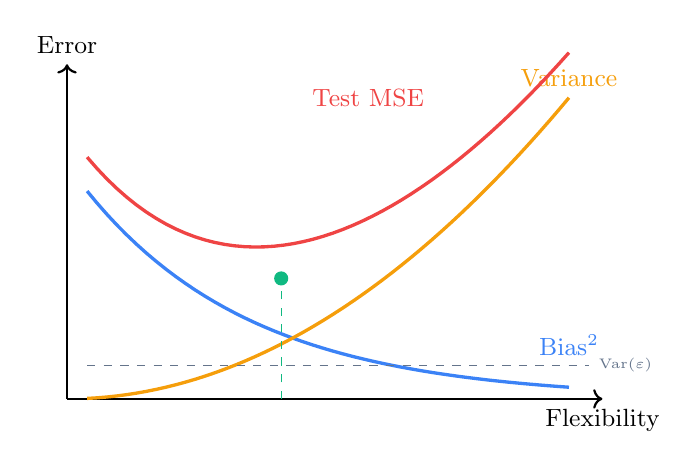
\begin{tikzpicture}[scale=0.85]
  \draw[->, thick] (0,0) -- (8,0) node[below] {\small Flexibility};
  \draw[->, thick] (0,0) -- (0,5) node[above] {\small Error};

  % Bias^2 - decreasing
  \draw[accent, very thick, domain=0.3:7.5, samples=50] plot (\x, {3.5*exp(-0.4*\x)});
  \node[accent] at (7.5, 0.8) {\small Bias$^2$};

  % Variance - increasing
  \draw[amber, very thick, domain=0.3:7.5, samples=50] plot (\x, {0.08*\x*\x});
  \node[amber] at (7.5, 4.8) {\small Variance};

  % Test MSE (sum) - U-shape
  \draw[softred, very thick, domain=0.3:7.5, samples=50] plot (\x, {3.5*exp(-0.4*\x) + 0.08*\x*\x + 0.5});
  \node[softred] at (4.5, 4.5) {\small Test MSE};

  % Irreducible
  \draw[muted, dashed] (0.3, 0.5) -- (7.8, 0.5);
  \node[muted, right] at (7.8, 0.5) {\tiny $\text{Var}(\varepsilon)$};

  % Optimal
  \draw[softgreen, dashed] (3.2, 0) -- (3.2, 1.8);
  \fill[softgreen] (3.2, 1.8) circle (3pt);
\end{tikzpicture}
\end{center}

\textbf{Key insight:} We can never observe this decomposition in practice!\\
$\Rightarrow$ Use \textbf{cross-validation} (Chapter~5) to estimate test MSE.
\end{frame}


\begin{frame}{Supervised vs.\ Unsupervised}
\begin{columns}
\column{0.48\textwidth}
\textbf{\textcolor{accent}{Supervised}}

For each $x_i$ we observe $y_i$

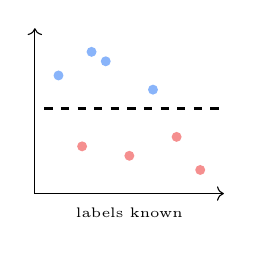
\begin{tikzpicture}[scale=0.6]
  \fill[accent!60] (0.5,2.5) circle (3pt); \fill[softred!60] (1,1) circle (3pt);
  \fill[accent!60] (1.5,2.8) circle (3pt); \fill[softred!60] (2,0.8) circle (3pt);
  \fill[accent!60] (2.5,2.2) circle (3pt); \fill[softred!60] (3,1.2) circle (3pt);
  \fill[accent!60] (1.2,3.0) circle (3pt); \fill[softred!60] (3.5,0.5) circle (3pt);
  \draw[thick, dashed] (0.2, 1.8) -- (4, 1.8);
  \draw[->] (0,0) -- (4,0); \draw[->] (0,0) -- (0,3.5);
  \node at (2, -0.4) {\tiny labels known};
\end{tikzpicture}

\vspace{0.3em}
Regression, Classification

\column{0.48\textwidth}
\textbf{\textcolor{softgreen}{Unsupervised}}

Only $x_i$, no $y_i$

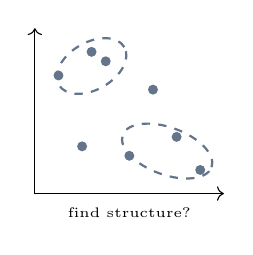
\begin{tikzpicture}[scale=0.6]
  \fill[muted] (0.5,2.5) circle (3pt); \fill[muted] (1,1) circle (3pt);
  \fill[muted] (1.5,2.8) circle (3pt); \fill[muted] (2,0.8) circle (3pt);
  \fill[muted] (2.5,2.2) circle (3pt); \fill[muted] (3,1.2) circle (3pt);
  \fill[muted] (1.2,3.0) circle (3pt); \fill[muted] (3.5,0.5) circle (3pt);
  \draw[->] (0,0) -- (4,0); \draw[->] (0,0) -- (0,3.5);
  \node at (2, -0.4) {\tiny find structure?};
  \draw[muted, thick, dashed, rotate around={30:(1.2,2.7)}] (1.2, 2.7) ellipse (0.8 and 0.5);
  \draw[muted, thick, dashed, rotate around={-20:(2.8,0.9)}] (2.8, 0.9) ellipse (1.0 and 0.5);
\end{tikzpicture}

\vspace{0.3em}
PCA, Clustering (Week 10)
\end{columns}
\end{frame}


\begin{frame}{Regression vs.\ Classification}
\begin{columns}
\column{0.48\textwidth}
\textbf{Regression:} $Y$ is quantitative

$$Y \in \mathbb{R}$$

Examples: price, salary, mpg, sales

\vspace{0.5em}
Method: Linear Regression

\column{0.48\textwidth}
\textbf{Classification:} $Y$ is categorical

$$Y \in \{0, 1\} \text{ or } \{A, B, C\}$$

Examples: spam/not, cancer type

\vspace{0.5em}
Method: Logistic Regression (Week 2)
\end{columns}

\vspace{1em}
\centering
\fbox{\parbox{0.7\textwidth}{\centering
The \textbf{predictor type} (qualitative/quantitative) matters less.\\
Most methods handle both.}}
\end{frame}


\begin{frame}{KNN Classifier: Intuition}
\begin{columns}
\column{0.45\textwidth}
\textbf{Algorithm:}
\begin{enumerate}
  \item Pick a new point $x_0$
  \item Find $K$ nearest neighbors
  \item Majority vote $\Rightarrow$ class
\end{enumerate}

$$P(Y = j \mid X = x_0) = \frac{1}{K}\sum_{i \in \mathcal{N}_0} \mathbf{1}(y_i = j)$$

\column{0.5\textwidth}
\textbf{Example:} $K = 3$

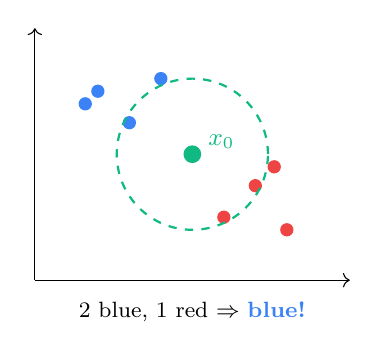
\begin{tikzpicture}[scale=0.8]
  \draw[->] (0,0) -- (5,0); \draw[->] (0,0) -- (0,4);
  % Blue class
  \fill[accent] (1,3) circle (3pt); \fill[accent] (1.5,2.5) circle (3pt);
  \fill[accent] (2,3.2) circle (3pt); \fill[accent] (0.8,2.8) circle (3pt);
  % Red class
  \fill[softred] (3,1) circle (3pt); \fill[softred] (3.5,1.5) circle (3pt);
  \fill[softred] (4,0.8) circle (3pt); \fill[softred] (3.8,1.8) circle (3pt);
  % New point
  \fill[softgreen] (2.5,2) circle (4pt);
  \node[softgreen, right] at (2.6,2.2) {\small $x_0$};
  % Circle around neighbors
  \draw[softgreen, thick, dashed] (2.5,2) circle (1.2);
  \node at (2.5, -0.5) {\footnotesize 2 blue, 1 red $\Rightarrow$ \textcolor{accent}{\textbf{blue!}}};
\end{tikzpicture}
\end{columns}
\end{frame}


\begin{frame}{KNN: Effect of $K$}
\begin{columns}
\column{0.32\textwidth}
\centering
\textbf{\textcolor{softred}{$K = 1$}}

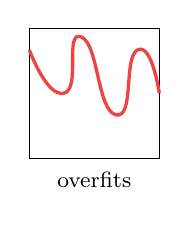
\begin{tikzpicture}[scale=0.55]
  \draw (0,0) rectangle (3,3);
  \draw[softred, very thick, smooth, tension=1.2] plot coordinates {(0,2.5)(0.8,1.5)(1.2,2.8)(2,1)(2.5,2.5)(3,1.5)};
  \node at (1.5, -0.5) {\footnotesize overfits};
\end{tikzpicture}

Training error = 0\\
\footnotesize Very wiggly boundary

\column{0.32\textwidth}
\centering
\textbf{\textcolor{softgreen}{$K = 10$}}

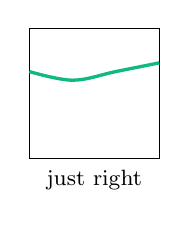
\begin{tikzpicture}[scale=0.55]
  \draw (0,0) rectangle (3,3);
  \draw[softgreen, very thick, smooth, tension=0.6] plot coordinates {(0,2)(1,1.8)(2,2)(3,2.2)};
  \node at (1.5, -0.5) {\footnotesize just right};
\end{tikzpicture}

Balanced\\
\footnotesize Smooth, generalizes well

\column{0.32\textwidth}
\centering
\textbf{\textcolor{muted}{$K = 100$}}

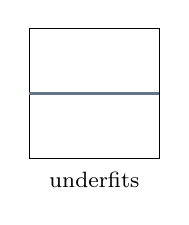
\begin{tikzpicture}[scale=0.55]
  \draw (0,0) rectangle (3,3);
  \draw[muted, very thick] (0,1.5) -- (3,1.5);
  \node at (1.5, -0.5) {\footnotesize underfits};
\end{tikzpicture}

Nearly linear\\
\footnotesize High bias
\end{columns}

\vspace{0.8em}
\centering
$\frac{1}{K}$ controls flexibility: small $K$ = flexible, large $K$ = rigid
\end{frame}


\begin{frame}{Chapter 2: Summary}
\begin{columns}
\column{0.48\textwidth}
\begin{itemize}
  \item $Y = f(X) + \varepsilon$
  \item Prediction vs.\ Inference
  \item Parametric vs.\ Non-parametric
  \item Bias--Variance trade-off
\end{itemize}

\column{0.48\textwidth}
\begin{itemize}
  \item MSE: training vs.\ test
  \item Flexibility $\leftrightarrow$ Interpretability
  \item No free lunch!
  \item KNN: $K$ controls smoothness
\end{itemize}
\end{columns}

\vspace{1em}
\centering
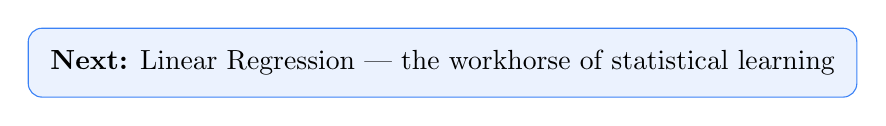
\begin{tikzpicture}
\node[fill=accent!10, rounded corners=5pt, inner sep=8pt, draw=accent] {
  \textbf{Next:} Linear Regression --- the workhorse of statistical learning
};
\end{tikzpicture}
\end{frame}


% ══════════════════════════════════════════════
% PART II: LINEAR REGRESSION
% ══════════════════════════════════════════════

\begin{frame}{Why Linear Regression?}
\begin{columns}
\column{0.55\textwidth}
\begin{itemize}
  \item Simple, interpretable, widely used
  \item \textbf{Foundation} for Lasso, Ridge, GAMs, \ldots
  \item Concepts (RSS, $R^2$, F-test) recur everywhere
  \item Benchmark for all fancier methods
\end{itemize}

\vspace{0.5em}
\textcolor{accent}{\textit{``Understand linear regression deeply\\before studying anything else.''}} --- ISLR

\column{0.4\textwidth}
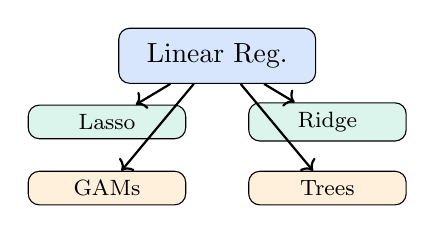
\begin{tikzpicture}[scale=0.7]
  \node[draw, fill=accent!20, rounded corners, minimum width=2.5cm, minimum height=0.7cm] (lr) at (0,0) {Linear Reg.};
  \node[draw, fill=softgreen!15, rounded corners, minimum width=2cm, font=\footnotesize] (la) at (-2,-1.2) {Lasso};
  \node[draw, fill=softgreen!15, rounded corners, minimum width=2cm, font=\footnotesize] (ri) at (2,-1.2) {Ridge};
  \node[draw, fill=amber!15, rounded corners, minimum width=2cm, font=\footnotesize] (ga) at (-2,-2.4) {GAMs};
  \node[draw, fill=amber!15, rounded corners, minimum width=2cm, font=\footnotesize] (tr) at (2,-2.4) {Trees};
  \draw[->, thick] (lr) -- (la);
  \draw[->, thick] (lr) -- (ri);
  \draw[->, thick] (lr) -- (ga);
  \draw[->, thick] (lr) -- (tr);
\end{tikzpicture}
\end{columns}
\end{frame}


\begin{frame}{Simple Linear Regression}
\begin{columns}
\column{0.5\textwidth}
\textbf{Model:}
$$Y = \beta_0 + \beta_1 X + \varepsilon$$

$\beta_0$ = intercept (value of $Y$ when $X = 0$)

$\beta_1$ = slope (change in $Y$ per unit $X$)

\vspace{0.5em}
\textbf{Estimate:}
$$\hat{Y} = \hat{\beta}_0 + \hat{\beta}_1 X$$

\column{0.45\textwidth}
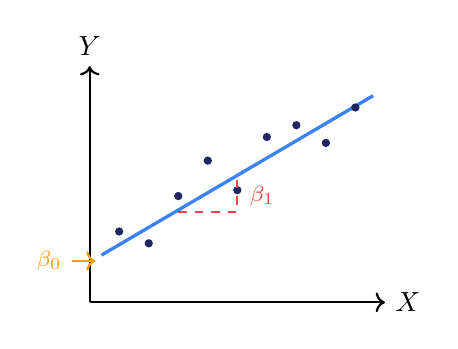
\begin{tikzpicture}[scale=0.75]
  \draw[->, thick] (0,0) -- (5,0) node[right] {$X$};
  \draw[->, thick] (0,0) -- (0,4) node[above] {$Y$};
  \draw[accent, very thick] (0.2, 0.8) -- (4.8, 3.5);
  % Points
  \foreach \x/\y in {0.5/1.2, 1/1.0, 1.5/1.8, 2/2.4, 2.5/1.9, 3/2.8, 3.5/3.0, 4/2.7, 4.5/3.3} {
    \fill[darkblue] (\x,\y) circle (2pt);
  }
  % Show slope
  \draw[softred, thick, dashed] (1.5, 1.53) -- (2.5, 1.53) -- (2.5, 2.1);
  \node[softred, right] at (2.55, 1.8) {\footnotesize $\beta_1$};
  % Show intercept
  \draw[amber, thick, <-] (0.1, 0.7) -- (-0.3, 0.7) node[left] {\footnotesize $\beta_0$};
\end{tikzpicture}
\end{columns}
\end{frame}


\begin{frame}{Least Squares: The Idea}
\begin{columns}
\column{0.5\textwidth}
Choose $\hat{\beta}_0, \hat{\beta}_1$ to minimize:

$$\text{RSS} = \sum_{i=1}^{n}(y_i - \hat{\beta}_0 - \hat{\beta}_1 x_i)^2$$

\vspace{0.3em}
\textbf{Minimize the sum of squared vertical distances}

\vspace{0.5em}
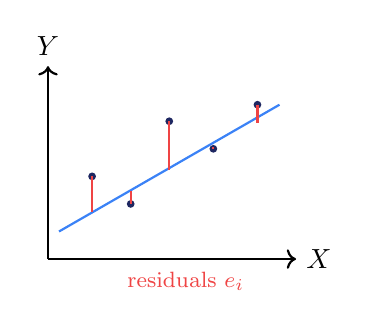
\begin{tikzpicture}[scale=0.7]
  \draw[->, thick] (0,0) -- (4.5,0) node[right] {$X$};
  \draw[->, thick] (0,0) -- (0,3.5) node[above] {$Y$};
  \draw[accent, thick] (0.2, 0.5) -- (4.2, 2.8);
  \foreach \x/\y/\yh in {0.8/1.5/0.85, 1.5/1.0/1.23, 2.2/2.5/1.61, 3.0/2.0/2.04, 3.8/2.8/2.47} {
    \fill[darkblue] (\x,\y) circle (2pt);
    \draw[softred, thick] (\x, \y) -- (\x, \yh);
  }
  \node[softred] at (2.5, -0.4) {\footnotesize residuals $e_i$};
\end{tikzpicture}

\column{0.45\textwidth}
\textbf{Closed-form solution:}

$$\hat{\beta}_1 = \frac{\sum_i(x_i - \bar{x})(y_i - \bar{y})}{\sum_i(x_i - \bar{x})^2}$$

$$\hat{\beta}_0 = \bar{y} - \hat{\beta}_1 \bar{x}$$

\vspace{0.5em}
\textit{The line always passes through $(\bar{x}, \bar{y})$}
\end{columns}
\end{frame}


\begin{frame}{Least Squares: Worked Example}
\begin{columns}
\column{0.45\textwidth}
\textbf{Data:} 5 points

\begin{tabular}{cc}
\toprule
$x_i$ & $y_i$ \\
\midrule
1 & 2.1 \\
2 & 3.8 \\
3 & 5.2 \\
4 & 6.5 \\
5 & 8.1 \\
\bottomrule
\end{tabular}

\vspace{0.5em}
$\bar{x} = 3, \quad \bar{y} = 5.14$

\column{0.5\textwidth}
\textbf{Computation:}

$\sum(x_i - \bar{x})(y_i - \bar{y}) = 11.9$

$\sum(x_i - \bar{x})^2 = 10$

$$\hat{\beta}_1 = \frac{11.9}{10} = 1.19$$
$$\hat{\beta}_0 = 5.14 - 1.19 \times 3 = 1.57$$

\vspace{0.3em}
$\hat{Y} = 1.57 + 1.19X$

\vspace{0.3em}
\textit{Each unit of $X$ $\Rightarrow$ $Y$ increases by 1.19}
\end{columns}
\end{frame}


\begin{frame}{How Good Is $\hat{\beta}_1$? Standard Errors}
\begin{columns}
\column{0.55\textwidth}
Different samples $\Rightarrow$ different $\hat{\beta}_1$

\vspace{0.3em}
\textbf{Standard Error} quantifies this variability:

$$\text{SE}(\hat{\beta}_1)^2 = \frac{\sigma^2}{\sum_i(x_i - \bar{x})^2}$$

$$\text{SE}(\hat{\beta}_0)^2 = \sigma^2\left[\frac{1}{n} + \frac{\bar{x}^2}{\sum_i(x_i - \bar{x})^2}\right]$$

\vspace{0.3em}
where $\sigma^2 \approx \text{RSE}^2 = \frac{\text{RSS}}{n-2}$

\column{0.4\textwidth}
\textbf{SE is smaller when:}

\begin{itemize}
  \item $n$ is larger
  \item $x_i$'s are more spread out
  \item $\sigma^2$ (noise) is smaller
\end{itemize}

\vspace{0.5em}
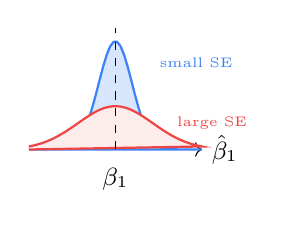
\begin{tikzpicture}[scale=0.55]
  \draw[->] (-2,0) -- (2,0) node[right] {\small $\hat{\beta}_1$};
  \draw[fill=accent!20, draw=accent, thick, domain=-2:2, samples=50] plot (\x, {2.5*exp(-\x*\x/0.3)}) -- (-2,0);
  \draw[fill=softred!10, draw=softred, thick, domain=-2:2, samples=50] plot (\x, {1.0*exp(-\x*\x/1.5)}) -- (-2,0);
  \draw[dashed] (0,0) -- (0,2.8);
  \node[accent, right] at (0.8, 2.0) {\tiny small SE};
  \node[softred, right] at (1.2, 0.6) {\tiny large SE};
  \node[below] at (0, -0.2) {\small $\beta_1$};
\end{tikzpicture}
\end{columns}
\end{frame}


\begin{frame}{Hypothesis Test: Is $X$ Related to $Y$?}

$$H_0: \beta_1 = 0 \quad \text{(no relationship)}$$
$$H_a: \beta_1 \neq 0 \quad \text{(some relationship)}$$

\vspace{0.5em}
\textbf{Test statistic:}
$$t = \frac{\hat{\beta}_1}{\text{SE}(\hat{\beta}_1)} \sim t_{n-2} \quad \text{under } H_0$$

\vspace{0.5em}
\begin{columns}
\column{0.5\textwidth}
\textbf{Example:}

$\hat{\beta}_1 = 0.0475$, $\text{SE} = 0.0027$

$t = 0.0475/0.0027 = 17.67$

$p\text{-value} < 0.0001$

\textcolor{softgreen}{\textbf{Reject $H_0$!}} Strong evidence.

\column{0.45\textwidth}
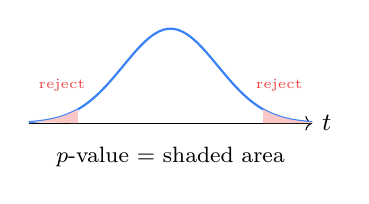
\begin{tikzpicture}[scale=0.6]
  \draw[->] (-3,0) -- (3,0) node[right] {\small $t$};
  \draw[accent, thick, domain=-3:3, samples=60] plot (\x, {2*exp(-\x*\x/2)});
  \fill[softred!30, domain=-3:-1.96, samples=30] plot (\x, {2*exp(-\x*\x/2)}) -- (-1.96,0);
  \fill[softred!30, domain=1.96:3, samples=30] plot (\x, {2*exp(-\x*\x/2)}) -- (3,0) -- (1.96,0);
  \node[softred] at (2.3, 0.8) {\tiny reject};
  \node[softred] at (-2.3, 0.8) {\tiny reject};
  \node[below] at (0, -0.3) {\footnotesize $p$-value = shaded area};
\end{tikzpicture}
\end{columns}
\end{frame}


\begin{frame}{Confidence Intervals}

\textbf{95\% CI for $\beta_1$:}
$$\hat{\beta}_1 \pm 2 \cdot \text{SE}(\hat{\beta}_1)$$

\vspace{0.3em}
\begin{columns}
\column{0.5\textwidth}
\textbf{Interpretation:}

In repeated sampling, 95\% of such intervals contain the true $\beta_1$

\vspace{0.5em}
\textbf{Example:}

$\hat{\beta}_1 = 0.0475 \pm 2(0.0027)$

$= [0.0421, \; 0.0529]$

\vspace{0.3em}
\textcolor{softgreen}{Does not contain 0} $\Rightarrow$ significant

\column{0.45\textwidth}
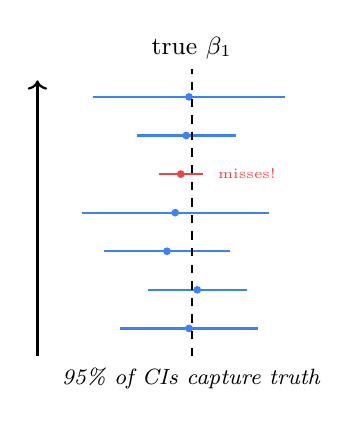
\begin{tikzpicture}[scale=0.7]
  \draw[thick, ->] (0,0) -- (0,5);
  \foreach \y/\l/\r/\c in {0.5/1.5/4.0/accent, 1.2/2.0/3.8/accent, 1.9/1.2/3.5/accent, 2.6/0.8/4.2/accent, 3.3/2.2/3.0/softred, 4.0/1.8/3.6/accent, 4.7/1.0/4.5/accent} {
    \draw[\c, thick] (\l, \y) -- (\r, \y);
    \fill[\c] ({(\l+\r)/2}, \y) circle (2pt);
  }
  \draw[dashed, thick] (2.8, 0) -- (2.8, 5.2) node[above] {\small true $\beta_1$};
  \node[softred, right] at (3.1, 3.3) {\tiny misses!};
  \node at (2.8, -0.4) {\footnotesize \textit{95\% of CIs capture truth}};
\end{tikzpicture}
\end{columns}
\end{frame}


\begin{frame}{Model Accuracy: RSE and $R^2$}
\begin{columns}
\column{0.48\textwidth}
\textbf{RSE} (Residual Standard Error):
$$\text{RSE} = \sqrt{\frac{\text{RSS}}{n - 2}}$$

\begin{itemize}
  \item In units of $Y$
  \item ``Typical prediction error''
  \item \textit{Advertising:} RSE $= 3.26$
  \item Average sales $= 14$ $\Rightarrow$ 23\% error
\end{itemize}

\column{0.48\textwidth}
\textbf{$R^2$} (Proportion of variance explained):
$$R^2 = 1 - \frac{\text{RSS}}{\text{TSS}} = 1 - \frac{\sum(y_i - \hat{y}_i)^2}{\sum(y_i - \bar{y})^2}$$

\begin{itemize}
  \item $R^2 \in [0, 1]$
  \item $R^2 = 0$: model = $\bar{y}$
  \item $R^2 = 1$: perfect fit
  \item In SLR: $R^2 = r_{XY}^2$
\end{itemize}
\end{columns}
\end{frame}


\begin{frame}{$R^2$: Visual Intuition}

\begin{center}
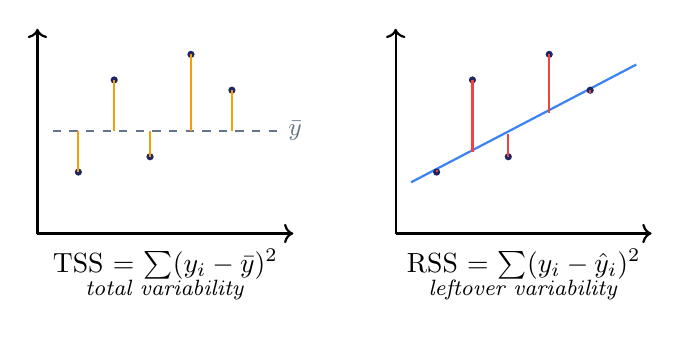
\begin{tikzpicture}[scale=0.65]
  % TSS picture
  \begin{scope}[xshift=0cm]
    \draw[->, thick] (0,0) -- (5,0); \draw[->, thick] (0,0) -- (0,4);
    \draw[muted, thick, dashed] (0.3, 2) -- (4.7, 2) node[right] {\small $\bar{y}$};
    \foreach \x/\y in {0.8/1.2, 1.5/3.0, 2.2/1.5, 3.0/3.5, 3.8/2.8} {
      \fill[darkblue] (\x, \y) circle (2pt);
      \draw[amber, thick] (\x, \y) -- (\x, 2);
    }
    \node at (2.5, -0.6) {TSS = $\sum(y_i - \bar{y})^2$};
    \node at (2.5, -1.1) {\footnotesize \textit{total variability}};
  \end{scope}

  % RSS picture
  \begin{scope}[xshift=7cm]
    \draw[->, thick] (0,0) -- (5,0); \draw[->, thick] (0,0) -- (0,4);
    \draw[accent, thick] (0.3, 1.0) -- (4.7, 3.3);
    \foreach \x/\y/\yh in {0.8/1.2/1.25, 1.5/3.0/1.6, 2.2/1.5/1.95, 3.0/3.5/2.35, 3.8/2.8/2.75} {
      \fill[darkblue] (\x, \y) circle (2pt);
      \draw[softred, thick] (\x, \y) -- (\x, \yh);
    }
    \node at (2.5, -0.6) {RSS = $\sum(y_i - \hat{y}_i)^2$};
    \node at (2.5, -1.1) {\footnotesize \textit{leftover variability}};
  \end{scope}
\end{tikzpicture}
\end{center}

$$R^2 = 1 - \frac{\text{RSS}}{\text{TSS}} = \frac{\text{variability explained by model}}{\text{total variability}}$$
\end{frame}


\begin{frame}{Multiple Linear Regression}

$$Y = \beta_0 + \beta_1 X_1 + \beta_2 X_2 + \cdots + \beta_p X_p + \varepsilon$$

\vspace{0.5em}
\begin{columns}
\column{0.5\textwidth}
\textbf{Interpretation of $\beta_j$:}

Average change in $Y$ per unit change in $X_j$,\\
\textbf{holding all other $X_k$ fixed}

\vspace{0.5em}
\textbf{Advertising:}

$\text{Sales} = 2.94 + 0.046 \cdot \text{TV}$\\
$\phantom{\text{Sales} = {}} + 0.189 \cdot \text{Radio}$\\
$\phantom{\text{Sales} = {}} - 0.001 \cdot \text{News}$

\column{0.45\textwidth}
\textbf{Key results:}

\begin{tabular}{lrl}
\toprule
& $\hat{\beta}$ & $p$ \\
\midrule
TV & 0.046 & $<0.001$ \\
Radio & 0.189 & $<0.001$ \\
News & $-0.001$ & 0.86 \\
\bottomrule
\end{tabular}

\vspace{0.5em}
\textcolor{softred}{Newspaper not significant!}

\vspace{0.2em}
\footnotesize (Confounded with Radio: $r = 0.35$)
\end{columns}
\end{frame}


\begin{frame}{Why Newspaper Vanishes}
\begin{columns}
\column{0.48\textwidth}
\textbf{Simple regression:}
\begin{tabular}{lr}
\toprule
& $p$-value \\
\midrule
TV alone & $<0.001$ \\
Radio alone & $<0.001$ \\
\textcolor{softred}{News alone} & \textcolor{softred}{$<0.001$} \\
\bottomrule
\end{tabular}

\vspace{0.3em}
Newspaper seems important!

\column{0.48\textwidth}
\textbf{Multiple regression:}
\begin{tabular}{lr}
\toprule
& $p$-value \\
\midrule
TV & $<0.001$ \\
Radio & $<0.001$ \\
\textcolor{softred}{Newspaper} & \textcolor{softred}{$0.86$} \\
\bottomrule
\end{tabular}

\vspace{0.3em}
Not significant!
\end{columns}

\vspace{0.8em}
\centering
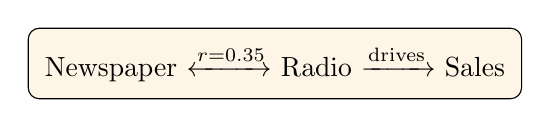
\begin{tikzpicture}
\node[draw, rounded corners, fill=amber!10, inner sep=6pt] {
  Newspaper $\xleftrightarrow{r=0.35}$ Radio $\xrightarrow{\text{drives}}$ Sales
};
\end{tikzpicture}

\vspace{0.3em}
\textit{Newspaper is a \textbf{proxy} for Radio, not an independent driver.}
\end{frame}


\begin{frame}{The F-Test: Overall Significance}

$$H_0: \beta_1 = \beta_2 = \cdots = \beta_p = 0$$

$$F = \frac{(\text{TSS} - \text{RSS})/p}{\text{RSS}/(n - p - 1)}$$

\vspace{0.3em}
\begin{columns}
\column{0.5\textwidth}
\textbf{Intuition:}
\begin{itemize}
  \item Numerator: improvement per predictor
  \item Denominator: residual noise per df
  \item Under $H_0$: $F \approx 1$
  \item Large $F$ $\Rightarrow$ predictors help!
\end{itemize}

\column{0.45\textwidth}
\textbf{Why not just t-tests?}

With $p = 100$ predictors and all $\beta_j = 0$:

\vspace{0.3em}
Expect $\sim5$ false positives at $\alpha = 0.05$!

\vspace{0.3em}
F-test avoids this \textbf{multiple testing} problem.
\end{columns}
\end{frame}


\begin{frame}{Qualitative Predictors: Dummy Variables}
\begin{columns}
\column{0.5\textwidth}
\textbf{Problem:} How to encode ``Region''?

\vspace{0.3em}
Create \textbf{indicator} (dummy) variables:

$$x_i = \begin{cases} 1 & \text{if female} \\ 0 & \text{if male}\end{cases}$$

\vspace{0.3em}
$k$ levels $\Rightarrow$ $k - 1$ dummies

\vspace{0.3em}
\textbf{R does this automatically!}

\texttt{lm(y \textasciitilde{} factor(region))}

\column{0.45\textwidth}
\textbf{Example:} 3 ethnicities

\vspace{0.3em}
\begin{tabular}{lcc}
\toprule
 & $x_1$ & $x_2$ \\
\midrule
African Am.\ & 0 & 0 \\
Asian & 1 & 0 \\
Caucasian & 0 & 1 \\
\bottomrule
\end{tabular}

\vspace{0.5em}
$\beta_0$ = mean for baseline

$\beta_1$ = Asian $-$ baseline

$\beta_2$ = Caucasian $-$ baseline
\end{columns}
\end{frame}


\begin{frame}{Interaction Terms: Synergy}
\begin{columns}
\column{0.55\textwidth}
\textbf{Without interaction:}
$$\text{Sales} = \beta_0 + \beta_1 \cdot \text{TV} + \beta_2 \cdot \text{Radio}$$

Effect of TV is \textbf{constant} regardless of Radio

\vspace{0.5em}
\textbf{With interaction:}
$$\text{Sales} = \beta_0 + \beta_1 \cdot \text{TV} + \beta_2 \cdot \text{Radio} + \beta_3 \cdot \text{TV} \times \text{Radio}$$

Effect of TV = $\beta_1 + \beta_3 \cdot \text{Radio}$

\textcolor{accent}{\textbf{More Radio $\Rightarrow$ TV is more effective!}}

\column{0.4\textwidth}
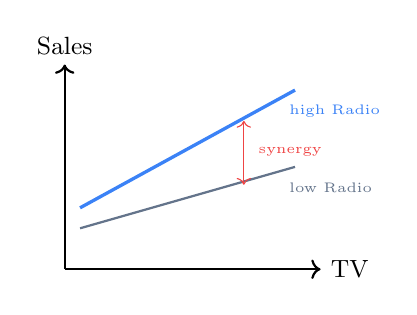
\begin{tikzpicture}[scale=0.65]
  \draw[->, thick] (0,0) -- (5,0) node[right] {\small TV};
  \draw[->, thick] (0,0) -- (0,4) node[above] {\small Sales};
  % Low Radio
  \draw[muted, thick] (0.3, 0.8) -- (4.5, 2.0);
  \node[muted, right] at (4.2, 1.6) {\tiny low Radio};
  % High Radio
  \draw[accent, very thick] (0.3, 1.2) -- (4.5, 3.5);
  \node[accent, right] at (4.2, 3.1) {\tiny high Radio};
  % Arrow showing difference
  \draw[<->, softred] (3.5, 1.65) -- (3.5, 2.9);
  \node[softred, right] at (3.6, 2.3) {\tiny synergy};
\end{tikzpicture}

\vspace{0.3em}
\footnotesize R: \texttt{lm(sales \textasciitilde{} TV * radio)}
\end{columns}
\end{frame}


\begin{frame}{Polynomial Regression}
\begin{columns}
\column{0.5\textwidth}
$$Y = \beta_0 + \beta_1 X + \beta_2 X^2 + \varepsilon$$

\vspace{0.3em}
Still \textbf{linear} in the parameters!

\vspace{0.3em}
\textbf{Auto data:}

\begin{tabular}{lc}
\toprule
Model & $R^2$ \\
\midrule
mpg $\sim$ hp & 0.606 \\
\textcolor{softgreen}{mpg $\sim$ hp + hp$^2$} & \textcolor{softgreen}{0.688} \\
mpg $\sim$ poly(hp, 5) & 0.693 \\
\bottomrule
\end{tabular}

\vspace{0.3em}
\footnotesize Quadratic captures most gain!

\column{0.45\textwidth}
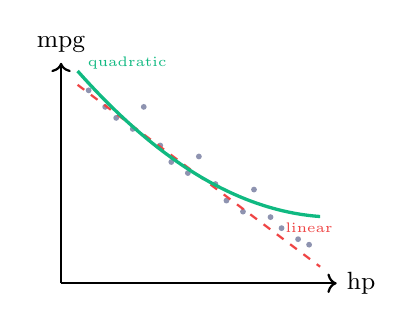
\begin{tikzpicture}[scale=0.7]
  \draw[->, thick] (0,0) -- (5,0) node[right] {\small hp};
  \draw[->, thick] (0,0) -- (0,4) node[above] {\small mpg};
  \foreach \x/\y in {0.5/3.5, 0.8/3.2, 1/3.0, 1.3/2.8, 1.5/3.2, 1.8/2.5, 2/2.2, 2.3/2.0, 2.5/2.3, 2.8/1.8, 3/1.5, 3.3/1.3, 3.5/1.7, 3.8/1.2, 4/1.0, 4.3/0.8, 4.5/0.7} {
    \fill[darkblue!50] (\x, \y) circle (1.5pt);
  }
  \draw[softred, thick, dashed] (0.3, 3.6) -- (4.7, 0.3);
  \draw[softgreen, very thick, domain=0.3:4.7, samples=40] plot (\x, {4.2 - 1.2*\x + 0.12*\x*\x});
  \node[softred] at (4.5, 1.0) {\tiny linear};
  \node[softgreen] at (1.2, 4.0) {\tiny quadratic};
\end{tikzpicture}
\end{columns}
\end{frame}


\begin{frame}{Potential Problems: Overview}

\begin{center}
\begin{tabular}{clll}
\toprule
\# & Problem & Diagnostic & Fix \\
\midrule
1 & Non-linearity & Residual plot & Polynomial/log \\
2 & Non-constant var. & Scale-Location & Transform $Y$ \\
3 & Correlated errors & Residuals vs.\ time & Time series \\
4 & Outliers & Studentized resid. & Investigate \\
5 & High leverage & Hat values $h_{ii}$ & Investigate \\
6 & Collinearity & VIF & Drop/combine \\
\bottomrule
\end{tabular}
\end{center}

\vspace{0.5em}
\centering
\textit{Always check residual plots before trusting results!}

\vspace{0.3em}
\textbf{Call to action:} \texttt{par(mfrow=c(2,2)); plot(fit)}
\end{frame}


\begin{frame}{Problem 1: Non-Linearity}
\begin{columns}
\column{0.48\textwidth}
\textbf{\textcolor{softgreen}{Good:} Random scatter}

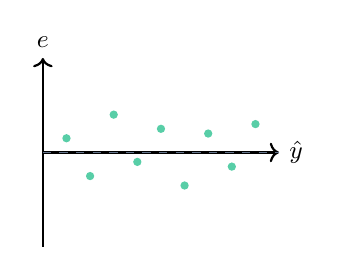
\begin{tikzpicture}[scale=0.6]
  \draw[->, thick] (0,0) -- (5,0) node[right] {\small $\hat{y}$};
  \draw[->, thick] (0,-2) -- (0,2) node[above] {\small $e$};
  \draw[muted, dashed] (0,0) -- (5,0);
  \foreach \x/\y in {0.5/0.3, 1/-0.5, 1.5/0.8, 2/-0.2, 2.5/0.5, 3/-0.7, 3.5/0.4, 4/-0.3, 4.5/0.6} {
    \fill[softgreen!70] (\x, \y) circle (2.5pt);
  }
\end{tikzpicture}

Assumptions satisfied!

\column{0.48\textwidth}
\textbf{\textcolor{softred}{Bad:} Curved pattern}

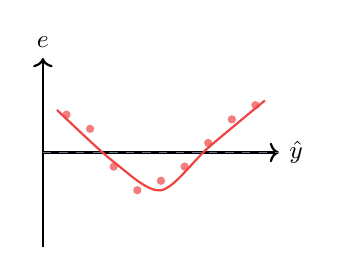
\begin{tikzpicture}[scale=0.6]
  \draw[->, thick] (0,0) -- (5,0) node[right] {\small $\hat{y}$};
  \draw[->, thick] (0,-2) -- (0,2) node[above] {\small $e$};
  \draw[muted, dashed] (0,0) -- (5,0);
  \foreach \x/\y in {0.5/0.8, 1/0.5, 1.5/-0.3, 2/-0.8, 2.5/-0.6, 3/-0.3, 3.5/0.2, 4/0.7, 4.5/1.0} {
    \fill[softred!70] (\x, \y) circle (2.5pt);
  }
  \draw[softred, thick, smooth, tension=0.5] plot coordinates {(0.3,0.9)(1.5,-0.2)(2.5,-0.8)(3.5,0.1)(4.7,1.1)};
\end{tikzpicture}

Non-linearity! Add $X^2$ term.
\end{columns}
\end{frame}


\begin{frame}{Problem 2: Heteroscedasticity}
\begin{columns}
\column{0.48\textwidth}
\textbf{\textcolor{softgreen}{Good:} Constant spread}

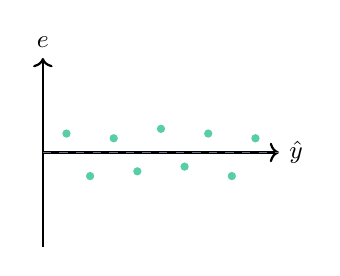
\begin{tikzpicture}[scale=0.6]
  \draw[->, thick] (0,0) -- (5,0) node[right] {\small $\hat{y}$};
  \draw[->, thick] (0,-2) -- (0,2) node[above] {\small $e$};
  \draw[muted, dashed] (0,0) -- (5,0);
  \foreach \x/\y in {0.5/0.4, 1/-0.5, 1.5/0.3, 2/-0.4, 2.5/0.5, 3/-0.3, 3.5/0.4, 4/-0.5, 4.5/0.3} {
    \fill[softgreen!70] (\x, \y) circle (2.5pt);
  }
\end{tikzpicture}

\column{0.48\textwidth}
\textbf{\textcolor{softred}{Bad:} Funnel shape}

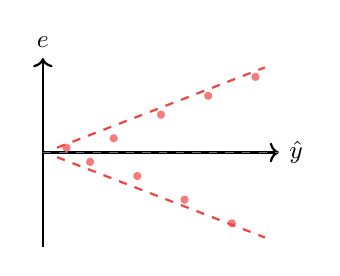
\begin{tikzpicture}[scale=0.6]
  \draw[->, thick] (0,0) -- (5,0) node[right] {\small $\hat{y}$};
  \draw[->, thick] (0,-2) -- (0,2) node[above] {\small $e$};
  \draw[muted, dashed] (0,0) -- (5,0);
  \foreach \x/\y in {0.5/0.1, 1/-0.2, 1.5/0.3, 2/-0.5, 2.5/0.8, 3/-1.0, 3.5/1.2, 4/-1.5, 4.5/1.6} {
    \fill[softred!70] (\x, \y) circle (2.5pt);
  }
  \draw[softred, thick, dashed] (0.3, 0.1) -- (4.7, 1.8);
  \draw[softred, thick, dashed] (0.3, -0.1) -- (4.7, -1.8);
\end{tikzpicture}

Variance grows! Try $\log(Y)$.
\end{columns}

\vspace{0.8em}
\centering
\textbf{Fix:} Transform response: $\log(Y)$, $\sqrt{Y}$, or use weighted least squares
\end{frame}


\begin{frame}{Problem 6: Collinearity}
\begin{columns}
\column{0.55\textwidth}
Two predictors highly correlated $\Rightarrow$\\
hard to separate their effects

\vspace{0.3em}
\textbf{Variance Inflation Factor:}
$$\text{VIF}(\hat{\beta}_j) = \frac{1}{1 - R^2_{X_j|X_{-j}}}$$

\begin{tabular}{cl}
\toprule
VIF & Interpretation \\
\midrule
1 & No collinearity \\
$1$--$5$ & Moderate \\
$5$--$10$ & \textcolor{amber}{High --- investigate} \\
$>10$ & \textcolor{softred}{Severe --- fix it!} \\
\bottomrule
\end{tabular}

\column{0.4\textwidth}
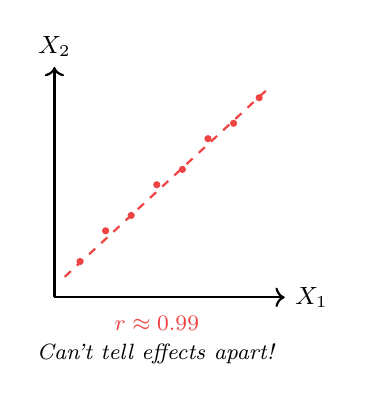
\begin{tikzpicture}[scale=0.65]
  \draw[->, thick] (0,0) -- (4.5,0) node[right] {\small $X_1$};
  \draw[->, thick] (0,0) -- (0,4.5) node[above] {\small $X_2$};
  % Correlated points
  \foreach \x/\y in {0.5/0.7, 1/1.3, 1.5/1.6, 2/2.2, 2.5/2.5, 3/3.1, 3.5/3.4, 4/3.9} {
    \fill[softred] (\x, \y) circle (2pt);
  }
  \draw[softred, thick, dashed] (0.2, 0.4) -- (4.2, 4.1);
  \node[softred] at (2, -0.5) {\footnotesize $r \approx 0.99$};
  \node at (2, -1.1) {\footnotesize \textit{Can't tell effects apart!}};
\end{tikzpicture}

\vspace{0.3em}
\footnotesize R: \texttt{car::vif(fit)}
\end{columns}
\end{frame}


\begin{frame}{Outliers vs.\ High Leverage}
\begin{columns}
\column{0.48\textwidth}
\textbf{Outlier:} unusual $y_i$

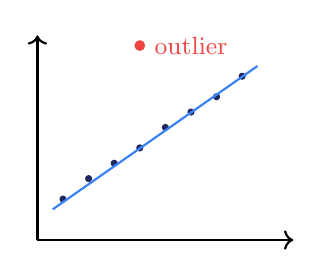
\begin{tikzpicture}[scale=0.65]
  \draw[->, thick] (0,0) -- (5,0); \draw[->, thick] (0,0) -- (0,4);
  \foreach \x/\y in {0.5/0.8, 1/1.2, 1.5/1.5, 2/1.8, 2.5/2.2, 3/2.5, 3.5/2.8, 4/3.2} {
    \fill[darkblue] (\x, \y) circle (2pt);
  }
  \fill[softred] (2, 3.8) circle (3pt);
  \node[softred, right] at (2.1, 3.8) {\small outlier};
  \draw[accent, thick] (0.3, 0.6) -- (4.3, 3.4);
\end{tikzpicture}

Little effect on slope,\\
but inflates RSE

\column{0.48\textwidth}
\textbf{High leverage:} unusual $x_i$

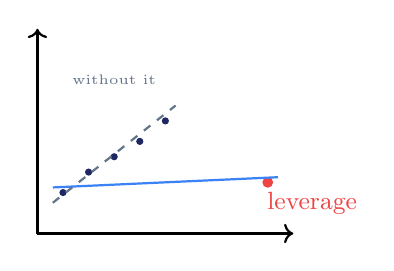
\begin{tikzpicture}[scale=0.65]
  \draw[->, thick] (0,0) -- (5,0); \draw[->, thick] (0,0) -- (0,4);
  \foreach \x/\y in {0.5/0.8, 1/1.2, 1.5/1.5, 2/1.8, 2.5/2.2} {
    \fill[darkblue] (\x, \y) circle (2pt);
  }
  \fill[softred] (4.5, 1.0) circle (3pt);
  \node[softred, right] at (4.3, 0.6) {\small leverage};
  \draw[accent, thick] (0.3, 0.9) -- (4.7, 1.1);
  \draw[muted, thick, dashed] (0.3, 0.6) -- (2.7, 2.5);
  \node[muted] at (1.5, 3.0) {\tiny without it};
\end{tikzpicture}

\textbf{Pulls the line!}\\
Detect: $h_{ii} \gg (p+1)/n$
\end{columns}
\end{frame}


\begin{frame}{$R^2$ Always Increases --- Adjusted $R^2$ Fixes This}

$$\text{Adj.\ } R^2 = 1 - \frac{\text{RSS}/(n-p-1)}{\text{TSS}/(n-1)}$$

\vspace{0.3em}
\begin{columns}
\column{0.5\textwidth}
\textbf{Example:}

\begin{tabular}{lcc}
\toprule
Model & $R^2$ & Adj.\ $R^2$ \\
\midrule
TV & 0.612 & 0.610 \\
TV + Radio & 0.897 & 0.896 \\
TV + Radio + News & 0.897 & 0.896 \\
\bottomrule
\end{tabular}

\vspace{0.3em}
Adding News: $R^2$ unchanged!

\column{0.45\textwidth}
\textbf{Key insight:}

$R^2$ \textbf{never} decreases when you add a predictor (even a useless one)

\vspace{0.3em}
Adj.\ $R^2$ \textbf{penalizes} for extra parameters $\Rightarrow$ can decrease

\vspace{0.3em}
Better for comparing models
\end{columns}
\end{frame}


\begin{frame}{Confidence vs.\ Prediction Intervals}
\begin{columns}
\column{0.48\textwidth}
\textbf{Confidence interval:}

For $E[Y \mid X = x_0]$

\vspace{0.2em}
Where the \textbf{average} response lies

\vspace{0.2em}
Narrower

\column{0.48\textwidth}
\textbf{Prediction interval:}

For a \textbf{new individual} $Y$ at $x_0$

\vspace{0.2em}
Includes $\text{Var}(\varepsilon)$

\vspace{0.2em}
Always wider!
\end{columns}

\vspace{0.5em}
\begin{center}
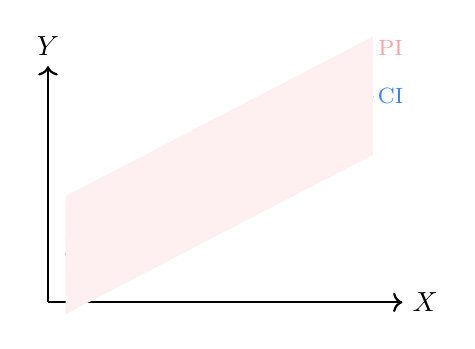
\begin{tikzpicture}[scale=0.75]
  \draw[->, thick] (0,0) -- (6,0) node[right] {$X$};
  \draw[->, thick] (0,0) -- (0,4) node[above] {$Y$};
  \draw[accent, very thick] (0.3, 0.8) -- (5.5, 3.5);
  % CI band
  \fill[accent!15] (0.3,0.5) -- (5.5,3.2) -- (5.5,3.8) -- (0.3,1.1) -- cycle;
  % PI band
  \fill[softred!8] (0.3,-0.2) -- (5.5,2.5) -- (5.5,4.5) -- (0.3,1.8) -- cycle;
  \node[accent] at (5.8, 3.5) {\footnotesize CI};
  \node[softred!50] at (5.8, 4.3) {\footnotesize PI};
\end{tikzpicture}
\end{center}
\end{frame}


\begin{frame}{OLS in Matrix Form}
\begin{columns}
\column{0.5\textwidth}
$$\mathbf{y} = \mathbf{X}\boldsymbol{\beta} + \boldsymbol{\varepsilon}$$

\vspace{0.3em}
where $\mathbf{X}$ is $n \times (p+1)$:
$$\mathbf{X} = \begin{pmatrix} 1 & x_{11} & \cdots & x_{1p} \\ 1 & x_{21} & \cdots & x_{2p} \\ \vdots & & & \vdots \\ 1 & x_{n1} & \cdots & x_{np} \end{pmatrix}$$

\column{0.45\textwidth}
\textbf{Solution:}
$$\hat{\boldsymbol{\beta}} = (\mathbf{X}^T\mathbf{X})^{-1}\mathbf{X}^T\mathbf{y}$$

\vspace{0.5em}
\textbf{Properties:}
\begin{itemize}
  \item Unbiased: $E[\hat{\boldsymbol{\beta}}] = \boldsymbol{\beta}$
  \item BLUE (Gauss-Markov)
  \item $\text{Var}(\hat{\boldsymbol{\beta}}) = \sigma^2(\mathbf{X}^T\mathbf{X})^{-1}$
\end{itemize}
\end{columns}
\end{frame}


\begin{frame}{The Hat Matrix: Who Influences Whom?}

$$\hat{\mathbf{y}} = \mathbf{H}\mathbf{y}, \qquad \mathbf{H} = \mathbf{X}(\mathbf{X}^T\mathbf{X})^{-1}\mathbf{X}^T$$

\vspace{0.5em}
\begin{columns}
\column{0.55\textwidth}
$h_{ii}$ = leverage of observation $i$

\begin{itemize}
  \item $\frac{1}{n} \leq h_{ii} \leq 1$
  \item Average: $\frac{p+1}{n}$
  \item Large $h_{ii}$ $\Rightarrow$ influential
\end{itemize}

\vspace{0.3em}
\textbf{Cook's distance} combines leverage \emph{and} residual:
$$D_i = \frac{e_i^2}{p \cdot \text{MSE}} \cdot \frac{h_{ii}}{(1-h_{ii})^2}$$

$D_i > 1$ $\Rightarrow$ influential point

\column{0.4\textwidth}
\textbf{Numerical example:}

$n = 50$, $p = 3$

Average leverage $= 4/50 = 0.08$

\vspace{0.3em}
Flag if $h_{ii} > 3 \times 0.08 = 0.24$

\vspace{0.3em}
\footnotesize R: \texttt{hatvalues(fit)}

\footnotesize R: \texttt{cooks.distance(fit)}
\end{columns}
\end{frame}


\begin{frame}{The 4 Diagnostic Plots in R}

\texttt{par(mfrow = c(2,2)); plot(fit)}

\vspace{0.5em}
\begin{columns}
\column{0.48\textwidth}
\begin{enumerate}
  \item \textbf{Residuals vs Fitted}
  \begin{itemize}
    \item[$\circ$] Checks linearity
    \item[$\circ$] Look for curves
  \end{itemize}

  \vspace{0.4em}
  \item \textbf{Normal Q-Q}
  \begin{itemize}
    \item[$\circ$] Checks normality
    \item[$\circ$] Points on diagonal = good
  \end{itemize}
\end{enumerate}

\column{0.48\textwidth}
\begin{enumerate}
  \setcounter{enumi}{2}
  \item \textbf{Scale-Location}
  \begin{itemize}
    \item[$\circ$] Checks constant variance
    \item[$\circ$] Horizontal band = good
  \end{itemize}

  \vspace{0.4em}
  \item \textbf{Residuals vs Leverage}
  \begin{itemize}
    \item[$\circ$] Finds influential points
    \item[$\circ$] Watch Cook's distance lines
  \end{itemize}
\end{enumerate}
\end{columns}

\vspace{0.5em}
\centering
\fbox{\textbf{Call to action:} Open \texttt{Lab\_Week1.R}, run lines 85--115}
\end{frame}


\begin{frame}{KNN Regression vs.\ Linear Regression}
\begin{columns}
\column{0.48\textwidth}
\textbf{KNN regression:}
$$\hat{f}(x_0) = \frac{1}{K}\sum_{i \in \mathcal{N}_0} y_i$$

Average of $K$ nearest neighbors

\vspace{0.3em}
\begin{itemize}
  \item[\textcolor{softgreen}{\textbullet}] No assumptions
  \item[\textcolor{softred}{\textbullet}] Curse of dimensionality!
\end{itemize}

\column{0.48\textwidth}
\textbf{When does each win?}

\vspace{0.3em}
\begin{tabular}{lcc}
\toprule
 & Linear & KNN \\
\midrule
Linear $f$ & \textcolor{softgreen}{\checkmark} & \\
Non-linear $f$ & & \textcolor{softgreen}{\checkmark} \\
Large $p$ & \textcolor{softgreen}{\checkmark} & \\
Small $p$ & & \textcolor{softgreen}{\checkmark} \\
\bottomrule
\end{tabular}
\end{columns}

\vspace{0.5em}
\centering
\textit{In high dimensions, even KNN struggles. Structure helps.}
\end{frame}


\begin{frame}{Curse of Dimensionality: A Numerical Example}
\begin{columns}
\column{0.55\textwidth}
\textbf{To capture 10\% of data} in KNN,\\
how far must we reach?

\vspace{0.3em}
Side length of hypercube:
$$\ell = 0.1^{1/p}$$

\begin{tabular}{cc}
\toprule
$p$ & $\ell$ \\
\midrule
1 & 0.10 \\
2 & 0.32 \\
5 & 0.63 \\
10 & \textcolor{softred}{0.80} \\
100 & \textcolor{softred}{0.98} \\
\bottomrule
\end{tabular}

\column{0.4\textwidth}
At $p = 10$: need 80\% of range!

\vspace{0.5em}
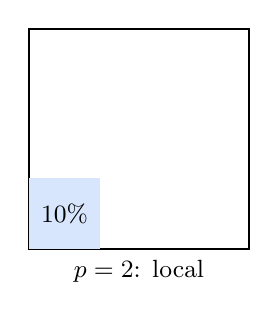
\begin{tikzpicture}[scale=0.7]
  \draw[thick] (0,0) rectangle (4,4);
  \fill[accent!20] (0,0) rectangle (1.3,1.3);
  \node at (0.65, 0.65) {\small 10\%};
  \node at (2, -0.4) {\small $p = 2$: local};
\end{tikzpicture}
\hspace{0.3cm}
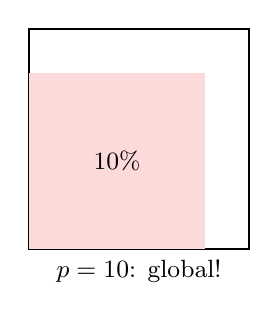
\begin{tikzpicture}[scale=0.7]
  \draw[thick] (0,0) rectangle (4,4);
  \fill[softred!20] (0,0) rectangle (3.2,3.2);
  \node at (1.6, 1.6) {\small 10\%};
  \node at (2, -0.4) {\small $p = 10$: global!};
\end{tikzpicture}
\end{columns}
\end{frame}


\begin{frame}{R Functions: Quick Reference}

\begin{center}
\begin{tabular}{ll}
\toprule
\texttt{lm(y \textasciitilde{} x1 + x2, data)} & Fit linear model \\
\texttt{summary(fit)} & Coefficients, $R^2$, F-test \\
\texttt{confint(fit)} & 95\% CIs \\
\texttt{predict(fit, newdata)} & Predictions \\
\texttt{plot(fit)} & 4 diagnostic plots \\
\texttt{car::vif(fit)} & VIF for collinearity \\
\texttt{anova(fit1, fit2)} & Compare nested models \\
\bottomrule
\end{tabular}
\end{center}

\vspace{0.3em}
\begin{center}
\begin{tabular}{ll}
\toprule
\texttt{y \textasciitilde{} x1 * x2} & Main effects + interaction \\
\texttt{y \textasciitilde{} poly(x, 2)} & Quadratic regression \\
\texttt{y \textasciitilde{} log(x)} & Log transform \\
\texttt{y \textasciitilde{} . - z} & All predictors except \texttt{z} \\
\bottomrule
\end{tabular}
\end{center}
\end{frame}


\begin{frame}{Key Formulas: Cheat Sheet}
\begin{columns}
\column{0.48\textwidth}
\textbf{Estimation:}
\begin{align*}
\hat{\beta}_1 &= \frac{\sum(x_i - \bar{x})(y_i - \bar{y})}{\sum(x_i - \bar{x})^2} \\[4pt]
\hat{\beta}_0 &= \bar{y} - \hat{\beta}_1 \bar{x} \\[4pt]
\hat{\boldsymbol{\beta}} &= (\mathbf{X}^T\mathbf{X})^{-1}\mathbf{X}^T\mathbf{y}
\end{align*}

\textbf{Quality:}
\begin{align*}
R^2 &= 1 - \text{RSS}/\text{TSS} \\
\text{RSE} &= \sqrt{\text{RSS}/(n-p-1)}
\end{align*}

\column{0.48\textwidth}
\textbf{Inference:}
\begin{align*}
t &= \hat{\beta}_j / \text{SE}(\hat{\beta}_j) \\[4pt]
F &= \frac{(\text{TSS}-\text{RSS})/p}{\text{RSS}/(n-p-1)} \\[4pt]
\text{CI} &: \hat{\beta}_j \pm t_{\alpha/2} \cdot \text{SE}
\end{align*}

\textbf{Diagnostics:}
\begin{align*}
\text{VIF}_j &= 1/(1 - R^2_{X_j|X_{-j}}) \\
h_{ii} &= [\mathbf{H}]_{ii}
\end{align*}
\end{columns}
\end{frame}


% ══════════════════════════════════════════════
% ADDITIONAL DEEP-DIVE SLIDES
% ══════════════════════════════════════════════

\begin{frame}{Think About It: What Does $\beta_1 = 0.046$ Mean?}
\begin{columns}
\column{0.5\textwidth}
\textbf{Advertising data:}

$\text{Sales} = 7.03 + 0.0475 \cdot \text{TV}$

\vspace{0.5em}
\textbf{Step by step:}
\begin{itemize}
  \item TV budget goes from \$100k to \$101k
  \item $\Delta\text{TV} = 1$ (thousand dollars)
  \item $\Delta\text{Sales} = 0.0475 \times 1 = 0.0475$
  \item That's 47.5 extra units sold
\end{itemize}

\vspace{0.3em}
\textcolor{accent}{\textit{Worth it? Depends on profit per unit!}}

\column{0.45\textwidth}
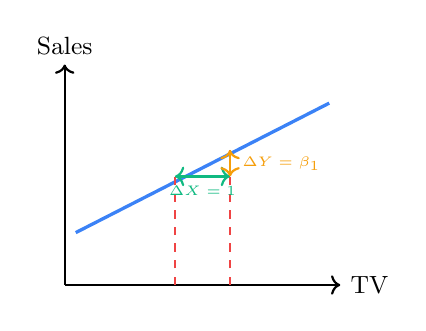
\begin{tikzpicture}[scale=0.7]
  \draw[->, thick] (0,0) -- (5,0) node[right] {\small TV};
  \draw[->, thick] (0,0) -- (0,4) node[above] {\small Sales};
  \draw[accent, very thick] (0.2, 0.95) -- (4.8, 3.3);
  \draw[softred, thick, dashed] (2, 0) -- (2, 1.97);
  \draw[softred, thick, dashed] (3, 0) -- (3, 2.45);
  \draw[<->, thick, softgreen] (2, 1.97) -- (3, 1.97);
  \draw[<->, thick, amber] (3, 1.97) -- (3, 2.45);
  \node[softgreen, below] at (2.5, 1.97) {\tiny $\Delta X = 1$};
  \node[amber, right] at (3.05, 2.2) {\tiny $\Delta Y = \beta_1$};
\end{tikzpicture}
\end{columns}
\end{frame}


\begin{frame}{The Intercept: Often Meaningless}
\begin{columns}
\column{0.55\textwidth}
$\hat{\beta}_0 = 7.03$ in Sales $\sim$ TV

\vspace{0.3em}
\textbf{Interpretation:}

Expected Sales when TV $= 0$

\vspace{0.3em}
\textbf{Problem:} Does TV $= 0$ make sense?

\begin{itemize}
  \item Sometimes yes (no advertising)
  \item Often extrapolation beyond data
  \item \texttt{mpg} at hp $= 0$? Nonsense!
\end{itemize}

\vspace{0.3em}
\textcolor{muted}{\textit{Focus on the slope, not the intercept}}

\column{0.4\textwidth}
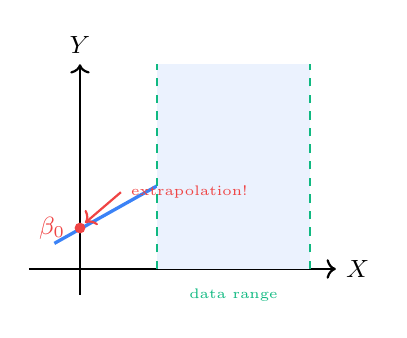
\begin{tikzpicture}[scale=0.65]
  \draw[->, thick] (-1,0) -- (5,0) node[right] {\small $X$};
  \draw[->, thick] (0,-0.5) -- (0,4) node[above] {\small $Y$};
  \draw[accent, very thick] (-0.5, 0.5) -- (4.5, 3.3);
  % Data range
  \fill[accent!10] (1.5, 0) rectangle (4.5, 4);
  \draw[softgreen, thick, dashed] (1.5, 0) -- (1.5, 4);
  \draw[softgreen, thick, dashed] (4.5, 0) -- (4.5, 4);
  \node[softgreen] at (3, -0.5) {\tiny data range};
  % Intercept
  \fill[softred] (0, 0.8) circle (3pt);
  \node[softred, left] at (-0.1, 0.8) {\small $\beta_0$};
  \draw[softred, thick, <-] (0.1, 0.9) -- (0.8, 1.5) node[right] {\tiny extrapolation!};
\end{tikzpicture}
\end{columns}
\end{frame}


\begin{frame}{Worked Example: Computing $R^2$}

\begin{columns}
\column{0.45\textwidth}
\begin{tabular}{cccc}
\toprule
$y_i$ & $\hat{y}_i$ & $(y_i - \bar{y})^2$ & $(y_i - \hat{y}_i)^2$ \\
\midrule
2 & 2.3 & 4 & 0.09 \\
4 & 3.8 & 0 & 0.04 \\
5 & 4.5 & 1 & 0.25 \\
3 & 3.0 & 1 & 0.00 \\
6 & 5.3 & 4 & 0.49 \\
\bottomrule
\end{tabular}

$\bar{y} = 4$

\column{0.5\textwidth}
$\text{TSS} = 4+0+1+1+4 = 10$

$\text{RSS} = 0.09+0.04+0.25+0+0.49 = 0.87$

\vspace{0.5em}
$$R^2 = 1 - \frac{0.87}{10} = 0.913$$

\vspace{0.3em}
\textcolor{softgreen}{\textbf{91.3\%}} of variability explained!

\vspace{0.3em}
$\text{RSE} = \sqrt{0.87/3} = 0.54$
\end{columns}
\end{frame}


\begin{frame}{$R^2$: What's a ``Good'' Value?}
\begin{columns}
\column{0.5\textwidth}
\textbf{It depends on the field!}

\vspace{0.3em}
\begin{tabular}{lc}
\toprule
Domain & Typical $R^2$ \\
\midrule
Physics experiments & $>0.99$ \\
Engineering & $0.8$--$0.95$ \\
Social sciences & $0.3$--$0.6$ \\
Finance (daily) & $0.01$--$0.05$ \\
\bottomrule
\end{tabular}

\vspace{0.5em}
$R^2 = 0.05$ can be \textbf{valuable} in trading!

\column{0.45\textwidth}
\textbf{Common mistakes:}

\begin{itemize}
  \item $R^2$ close to 1 does NOT mean model is correct
  \item High $R^2$ can come from overfitting
  \item Low $R^2$ doesn't mean $X$ is irrelevant
  \item Always pair with residual diagnostics
\end{itemize}
\end{columns}
\end{frame}


\begin{frame}{Residual = Observed $-$ Predicted}

$$e_i = y_i - \hat{y}_i$$

\begin{columns}
\column{0.5\textwidth}
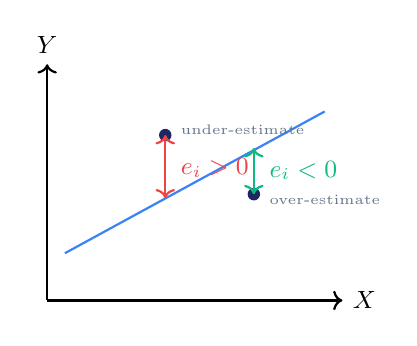
\begin{tikzpicture}[scale=0.75]
  \draw[->, thick] (0,0) -- (5,0) node[right] {\small $X$};
  \draw[->, thick] (0,0) -- (0,4) node[above] {\small $Y$};
  \draw[accent, thick] (0.3, 0.8) -- (4.7, 3.2);

  % Point above line
  \fill[darkblue] (2, 2.8) circle (3pt);
  \draw[softred, thick, <->] (2, 2.8) -- (2, 1.73);
  \node[softred, right] at (2.1, 2.25) {\small $e_i > 0$};
  \node[muted, right] at (2.1, 2.9) {\tiny under-estimate};

  % Point below line
  \fill[darkblue] (3.5, 1.8) circle (3pt);
  \draw[softgreen, thick, <->] (3.5, 1.8) -- (3.5, 2.58);
  \node[softgreen, right] at (3.6, 2.2) {\small $e_i < 0$};
  \node[muted, right] at (3.6, 1.7) {\tiny over-estimate};
\end{tikzpicture}

\column{0.45\textwidth}
\textbf{Key properties:}

\begin{itemize}
  \item $\sum e_i = 0$ (by construction)
  \item $\sum x_i e_i = 0$
  \item $\text{RSS} = \sum e_i^2$
\end{itemize}

\vspace{0.5em}
\textit{Residuals tell us what the model missed!}
\end{columns}
\end{frame}


\begin{frame}{From Correlation to Regression}

\begin{columns}
\column{0.48\textwidth}
\textbf{Correlation:}
$$r = \frac{\sum(x_i - \bar{x})(y_i - \bar{y})}{\sqrt{\sum(x_i-\bar{x})^2 \cdot \sum(y_i-\bar{y})^2}}$$

$r \in [-1, 1]$

Measures \textit{strength} and \textit{direction}

\column{0.48\textwidth}
\textbf{Regression slope:}
$$\hat{\beta}_1 = r \cdot \frac{s_Y}{s_X}$$

\vspace{0.3em}
Same sign as $r$, but scaled!

\vspace{0.3em}
$r = 0.78$ (TV vs Sales)

$\hat{\beta}_1 = 0.0475$ (in original units)
\end{columns}

\vspace{0.8em}
\centering
In SLR: $\quad R^2 = r^2 = 0.78^2 = 0.61$ \quad\textcolor{softgreen}{\checkmark}
\end{frame}


\begin{frame}{The $t$-Distribution: Why Not Normal?}

\begin{columns}
\column{0.55\textwidth}
We estimate $\sigma^2$ with RSE$^2$

This adds uncertainty $\Rightarrow$ heavier tails

$$t = \frac{\hat{\beta}_1}{\text{SE}(\hat{\beta}_1)} \sim t_{n-2}$$

\vspace{0.3em}
For large $n$: $t_{n-2} \approx N(0,1)$

For small $n$: $t_{n-2}$ has fatter tails\\
$\Rightarrow$ wider CIs, harder to reject $H_0$

\column{0.4\textwidth}
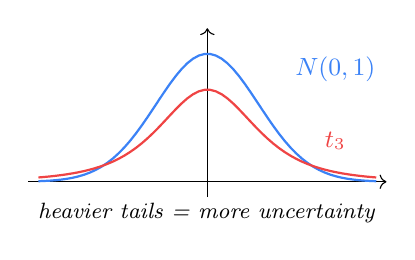
\begin{tikzpicture}[scale=0.65]
  \draw[->] (-3.5,0) -- (3.5,0);
  \draw[->] (0,-0.3) -- (0,3);
  % Normal
  \draw[accent, thick, domain=-3.3:3.3, samples=60] plot (\x, {2.5*exp(-\x*\x/2)});
  % t with df=3
  \draw[softred, thick, domain=-3.3:3.3, samples=60] plot (\x, {1.8/(1+\x*\x/3)^2});
  \node[accent] at (2.5, 2.2) {\small $N(0,1)$};
  \node[softred] at (2.5, 0.8) {\small $t_3$};
  \node at (0, -0.6) {\footnotesize \textit{heavier tails = more uncertainty}};
\end{tikzpicture}
\end{columns}
\end{frame}


\begin{frame}{Worked Example: Hypothesis Test}

\textbf{Advertising:} Is TV related to Sales?

\vspace{0.3em}
\begin{columns}
\column{0.5\textwidth}
$\hat{\beta}_1 = 0.0475$

$\text{SE}(\hat{\beta}_1) = 0.0027$

$$t = \frac{0.0475}{0.0027} = 17.67$$

$n - 2 = 198$ degrees of freedom

$p$-value $< 2 \times 10^{-16}$

\column{0.45\textwidth}
\textbf{Decision:}

$|t| = 17.67 \gg 1.97$ (critical value)

\vspace{0.3em}
\textcolor{softgreen}{\textbf{Reject $H_0$}}

\vspace{0.3em}
Extremely strong evidence that\\
TV budget is related to Sales

\vspace{0.3em}
\footnotesize (The chance of seeing $t = 17.67$ if $\beta_1 = 0$ is essentially zero)
\end{columns}
\end{frame}


\begin{frame}{Multiple Regression: Why Not Just Run Separate SLRs?}

\begin{columns}
\column{0.55\textwidth}
\textbf{Problem:}

Running mpg $\sim$ horsepower and\\
mpg $\sim$ weight separately

$\Rightarrow$ \textbf{cannot} hold other variables fixed

$\Rightarrow$ confounding!

\vspace{0.5em}
\textbf{MLR advantage:}

Each $\hat{\beta}_j$ is the \textbf{partial effect}\\
of $X_j$ after removing the effect\\
of all other predictors

\column{0.4\textwidth}
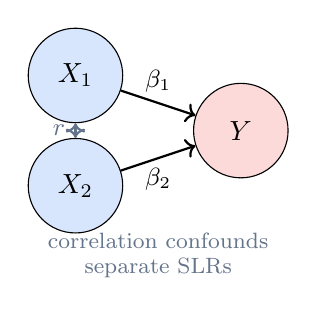
\begin{tikzpicture}[scale=0.7]
  \node[draw, circle, fill=accent!20, minimum size=1.2cm] (x1) at (0, 2) {$X_1$};
  \node[draw, circle, fill=accent!20, minimum size=1.2cm] (x2) at (0, 0) {$X_2$};
  \node[draw, circle, fill=softred!20, minimum size=1.2cm] (y) at (3, 1) {$Y$};
  \draw[->, thick] (x1) -- (y) node[midway, above] {\small $\beta_1$};
  \draw[->, thick] (x2) -- (y) node[midway, below] {\small $\beta_2$};
  \draw[<->, thick, muted, dashed] (x1) -- (x2) node[midway, left] {\small $r$};
  \node[muted] at (1.5, -1) {\footnotesize correlation confounds};
  \node[muted] at (1.5, -1.5) {\footnotesize separate SLRs};
\end{tikzpicture}
\end{columns}
\end{frame}


\begin{frame}{F-Test: Worked Example}

\textbf{Advertising:} Sales $\sim$ TV + Radio + Newspaper

\vspace{0.3em}
$n = 200$, $p = 3$

\begin{columns}
\column{0.5\textwidth}
$\text{TSS} = 5417.15$

$\text{RSS} = 556.91$

$$F = \frac{(5417.15 - 556.91)/3}{556.91/(200-3-1)}$$

$$= \frac{1620.1}{2.84} = 570.3$$

\column{0.45\textwidth}
Under $H_0$: $F \sim F_{3, 196}$

\vspace{0.3em}
$F = 570.3 \gg 1$

$p$-value $< 10^{-16}$

\vspace{0.3em}
\textcolor{softgreen}{\textbf{At least one predictor matters!}}

\vspace{0.3em}
\footnotesize (But which ones? Check individual $t$-tests)
\end{columns}
\end{frame}


\begin{frame}{Interactions: Quantitative $\times$ Qualitative}

\begin{columns}
\column{0.5\textwidth}
\textbf{Without interaction:}

$Y = \beta_0 + \beta_1 X + \beta_2 D$

\vspace{0.2em}
Same slope, different intercepts

\vspace{0.8em}
\textbf{With interaction:}

$Y = \beta_0 + \beta_1 X + \beta_2 D + \beta_3 (X \cdot D)$

\vspace{0.2em}
Different slopes AND intercepts

\column{0.45\textwidth}
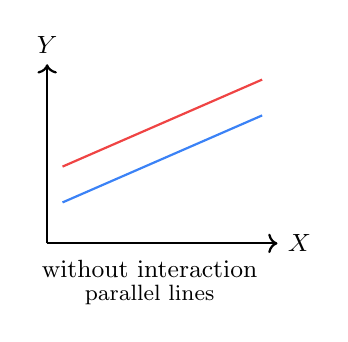
\begin{tikzpicture}[scale=0.65]
  \draw[->, thick] (0,0) -- (4.5,0) node[right] {\small $X$};
  \draw[->, thick] (0,0) -- (0,3.5) node[above] {\small $Y$};
  \draw[accent, thick] (0.3, 0.8) -- (4.2, 2.5);
  \draw[softred, thick] (0.3, 1.5) -- (4.2, 3.2);
  \node at (2, -0.5) {\small without interaction};
  \node at (2, -1.0) {\footnotesize parallel lines};
\end{tikzpicture}

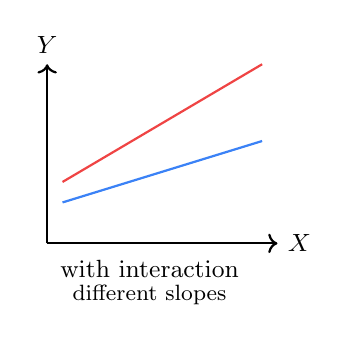
\begin{tikzpicture}[scale=0.65]
  \draw[->, thick] (0,0) -- (4.5,0) node[right] {\small $X$};
  \draw[->, thick] (0,0) -- (0,3.5) node[above] {\small $Y$};
  \draw[accent, thick] (0.3, 0.8) -- (4.2, 2.0);
  \draw[softred, thick] (0.3, 1.2) -- (4.2, 3.5);
  \node at (2, -0.5) {\small with interaction};
  \node at (2, -1.0) {\footnotesize different slopes};
\end{tikzpicture}
\end{columns}
\end{frame}


\begin{frame}{The Hierarchical Principle}

\textbf{Rule:} If an interaction $X_1 \times X_2$ is in the model,\\
keep both main effects $X_1$ and $X_2$.

\vspace{0.5em}
\begin{columns}
\column{0.5\textwidth}
\textcolor{softgreen}{\textbf{Correct:}}

$Y = \beta_0 + \beta_1 X_1 + \beta_2 X_2 + \beta_3 X_1 X_2$

\vspace{0.5em}
\textcolor{softred}{\textbf{Wrong:}}

$Y = \beta_0 + \beta_3 X_1 X_2$

\column{0.45\textwidth}
\textbf{Why?}

\begin{itemize}
  \item Removing $X_1$ changes meaning of $\beta_3$
  \item Interaction without main effects is hard to interpret
  \item Even if $\beta_1$ is not significant, keep it
\end{itemize}
\end{columns}
\end{frame}


\begin{frame}{Log Transformations: Three Scenarios}

\begin{center}
\begin{tabular}{lll}
\toprule
Model & Formula & Interpretation of $\beta_1$ \\
\midrule
Level-level & $Y = \beta_0 + \beta_1 X$ & $\Delta X = 1 \Rightarrow \Delta Y = \beta_1$ \\
Log-level & $\log Y = \beta_0 + \beta_1 X$ & $\Delta X = 1 \Rightarrow$ \%$\Delta Y \approx 100\beta_1$ \\
Level-log & $Y = \beta_0 + \beta_1 \log X$ & \%$\Delta X = 1 \Rightarrow \Delta Y \approx \beta_1/100$ \\
Log-log & $\log Y = \beta_0 + \beta_1 \log X$ & \textbf{Elasticity:} \%$\Delta X \Rightarrow$ \%$\Delta Y$ \\
\bottomrule
\end{tabular}
\end{center}

\vspace{0.5em}
\textbf{When to use $\log$:}
\begin{itemize}
  \item Skewed response (income, prices)
  \item Funnel-shaped residuals (heteroscedasticity)
  \item Multiplicative relationships
\end{itemize}
\end{frame}


\begin{frame}{Simpson's Paradox: A Warning}

\begin{columns}
\column{0.55\textwidth}
\textbf{The trap:}

A trend in subgroups can \textbf{reverse}\\
when groups are combined!

\vspace{0.3em}
\textbf{Example:}

Treatment appears harmful overall,\\
but is beneficial within each group

\vspace{0.3em}
\textbf{Cause:} Confounding variable\\
(group membership)

\vspace{0.3em}
\textcolor{softred}{\textbf{Lesson:} Always consider omitted variables}

\column{0.4\textwidth}
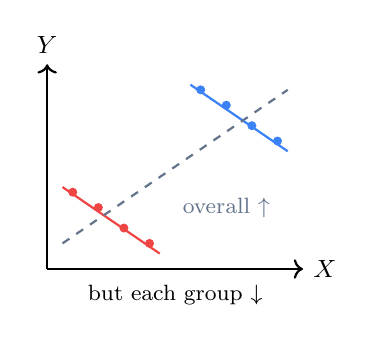
\begin{tikzpicture}[scale=0.65]
  \draw[->, thick] (0,0) -- (5,0) node[right] {\small $X$};
  \draw[->, thick] (0,0) -- (0,4) node[above] {\small $Y$};
  % Group 1 (upper)
  \foreach \x/\y in {3/3.5, 3.5/3.2, 4/2.8, 4.5/2.5} {
    \fill[accent] (\x, \y) circle (2.5pt);
  }
  \draw[accent, thick] (2.8, 3.6) -- (4.7, 2.3);
  % Group 2 (lower)
  \foreach \x/\y in {0.5/1.5, 1/1.2, 1.5/0.8, 2/0.5} {
    \fill[softred] (\x, \y) circle (2.5pt);
  }
  \draw[softred, thick] (0.3, 1.6) -- (2.2, 0.3);
  % Overall trend
  \draw[muted, thick, dashed] (0.3, 0.5) -- (4.7, 3.5);
  \node[muted] at (3.5, 1.2) {\footnotesize overall $\uparrow$};
  \node at (2.5, -0.5) {\footnotesize but each group $\downarrow$};
\end{tikzpicture}
\end{columns}
\end{frame}


\begin{frame}{Correlation $\neq$ Causation}

\begin{center}
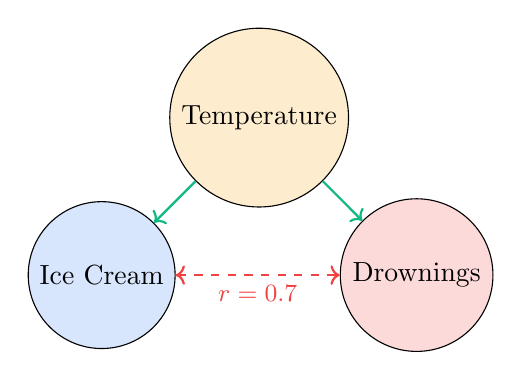
\begin{tikzpicture}[scale=0.8]
  \node[draw, circle, fill=accent!20, minimum size=1.5cm] (ice) at (0, 0) {Ice Cream};
  \node[draw, circle, fill=softred!20, minimum size=1.5cm] (drown) at (5, 0) {Drownings};
  \node[draw, circle, fill=amber!20, minimum size=1.5cm] (temp) at (2.5, 2.5) {Temperature};

  \draw[<->, thick, softred, dashed] (ice) -- (drown) node[midway, below] {\small $r = 0.7$};
  \draw[->, thick, softgreen] (temp) -- (ice);
  \draw[->, thick, softgreen] (temp) -- (drown);
\end{tikzpicture}
\end{center}

\vspace{0.5em}
\begin{itemize}
  \item Regression finds \textbf{associations}, not causes
  \item Confounders create spurious correlations
  \item Causation requires: experiments, randomization, or careful causal inference
\end{itemize}
\end{frame}


\begin{frame}{Extrapolation: Stay Within the Data Range}

\begin{columns}
\column{0.5\textwidth}
\textbf{Dangerous:}

Predicting outside the range of\\
observed $X$ values

\vspace{0.3em}
The linear relationship may not\\
hold beyond the data

\vspace{0.3em}
\textbf{Example:}

TV budget in data: \$0--\$300k

Predicting at \$500k?\\
\textcolor{softred}{Unreliable!}

\column{0.45\textwidth}
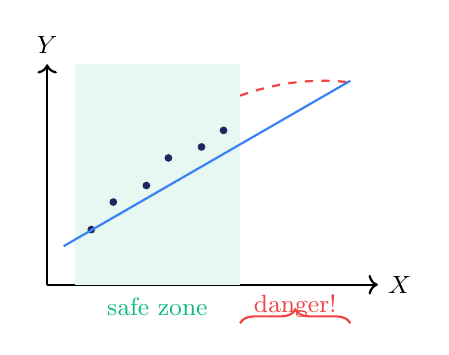
\begin{tikzpicture}[scale=0.7]
  \draw[->, thick] (0,0) -- (6,0) node[right] {\small $X$};
  \draw[->, thick] (0,0) -- (0,4) node[above] {\small $Y$};
  % Data range
  \fill[softgreen!10] (0.5, 0) rectangle (3.5, 4);
  \foreach \x/\y in {0.8/1.0, 1.2/1.5, 1.8/1.8, 2.2/2.3, 2.8/2.5, 3.2/2.8} {
    \fill[darkblue] (\x, \y) circle (2pt);
  }
  \draw[accent, thick] (0.3, 0.7) -- (5.5, 3.7);
  % True curve
  \draw[softred, thick, dashed, domain=3.5:5.5, samples=20] plot (\x, {0.7 + 1.2*\x - 0.12*\x*\x});
  \node[softgreen] at (2, -0.4) {\small safe zone};
  \node[softred] at (4.5, -0.4) {\small danger!};
  \draw[softred, thick, decorate, decoration={brace, amplitude=5pt}] (3.5, -0.7) -- (5.5, -0.7);
\end{tikzpicture}
\end{columns}
\end{frame}


\begin{frame}{Weighted Least Squares: When Variance Varies}

\begin{columns}
\column{0.5\textwidth}
\textbf{Standard OLS:}

Assumes $\text{Var}(\varepsilon_i) = \sigma^2$ for all $i$

\vspace{0.5em}
\textbf{WLS:}

Allows $\text{Var}(\varepsilon_i) = \sigma^2/w_i$

Minimize:
$$\sum_{i=1}^n w_i (y_i - \hat{\beta}_0 - \hat{\beta}_1 x_i)^2$$

\vspace{0.3em}
\footnotesize R: \texttt{lm(y \textasciitilde{} x, weights = w)}

\column{0.45\textwidth}
\textbf{Intuition:}

Give \textbf{more weight} to observations with smaller variance

\vspace{0.3em}
\textbf{Common case:}

$y_i$ is an average of $n_i$ observations

$\Rightarrow w_i = n_i$

\vspace{0.5em}
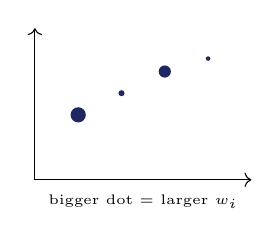
\begin{tikzpicture}[scale=0.55]
  \draw[->] (0,0) -- (5,0); \draw[->] (0,0) -- (0,3.5);
  \fill[darkblue] (1, 1.5) circle (5pt);
  \fill[darkblue] (2, 2.0) circle (2pt);
  \fill[darkblue] (3, 2.5) circle (4pt);
  \fill[darkblue] (4, 2.8) circle (1.5pt);
  \node at (2.5, -0.5) {\tiny bigger dot = larger $w_i$};
\end{tikzpicture}
\end{columns}
\end{frame}


\begin{frame}{Model Selection Preview: Which Predictors to Keep?}
\begin{columns}
\column{0.55\textwidth}
\textbf{With $p$ predictors:} $2^p$ possible models!

\vspace{0.3em}
\begin{tabular}{cl}
\toprule
$p$ & \# Models \\
\midrule
5 & 32 \\
10 & 1,024 \\
20 & \textcolor{softred}{1,048,576} \\
\bottomrule
\end{tabular}

\vspace{0.3em}
Can't check all! Need smart strategies.

\column{0.4\textwidth}
\textbf{Preview (Chapter 6):}

\begin{itemize}
  \item Forward selection
  \item Backward selection
  \item Best subset selection
  \item Lasso (automatic!)
\end{itemize}

\vspace{0.3em}
\textbf{Criteria:}

AIC, BIC, Adj.~$R^2$, $C_p$, CV
\end{columns}
\end{frame}


\begin{frame}{Reading the R Output: A Guided Tour}
\footnotesize
\begin{columns}
\column{0.48\textwidth}
\texttt{> summary(lm(sales \textasciitilde{} TV))}

\vspace{0.3em}
\begin{tabular}{lrrrr}
\toprule
 & Est. & SE & $t$ & $p$ \\
\midrule
Int & 7.03 & 0.46 & 15.4 & $<$0.001 \\
TV & 0.048 & 0.003 & 17.7 & $<$0.001 \\
\bottomrule
\end{tabular}

\vspace{0.3em}
RSE: 3.26 on 198 df

$R^2$: 0.612

Adj $R^2$: 0.610

F: 312.1, $p < 10^{-16}$

\column{0.48\textwidth}
\textbf{Read it like a story:}

\begin{enumerate}
  \item F-test: overall model significant?\\
    \textcolor{softgreen}{Yes!} ($p < 10^{-16}$)
  \item Coefficients: which matter?\\
    \textcolor{softgreen}{TV significant} ($p < 0.001$)
  \item $R^2$: how much explained?\\
    61\% of variance
  \item RSE: how big are errors?\\
    $\pm 3.26$ thousand units
\end{enumerate}
\end{columns}
\end{frame}


\begin{frame}{VIF: A Worked Example}
\begin{columns}
\column{0.55\textwidth}
\textbf{Auto data:} mpg $\sim$ cylinders + displacement + weight

\vspace{0.3em}
Step 1: Regress displacement on\\
cylinders and weight

$R^2_{\text{disp}|\text{others}} = 0.89$

\vspace{0.3em}
Step 2: Compute VIF

$$\text{VIF}_{\text{disp}} = \frac{1}{1 - 0.89} = 9.1$$

\vspace{0.3em}
\textcolor{softred}{VIF $> 5$ $\Rightarrow$ problematic collinearity!}

\column{0.4\textwidth}
\textbf{Typical Auto VIFs:}

\begin{tabular}{lr}
\toprule
Predictor & VIF \\
\midrule
cylinders & 9.1 \\
displacement & \textcolor{softred}{14.3} \\
horsepower & 8.7 \\
weight & \textcolor{softred}{10.8} \\
year & 1.2 \\
origin & 1.8 \\
\bottomrule
\end{tabular}

\vspace{0.2em}
\footnotesize year \& origin: no issue!
\end{columns}
\end{frame}


\begin{frame}{Overfitting: The Core Danger}
\begin{columns}
\column{0.48\textwidth}
\textbf{Underfitting:}

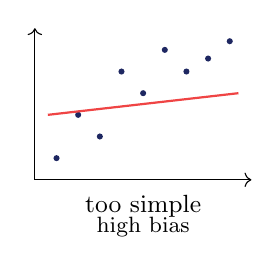
\begin{tikzpicture}[scale=0.55]
  \draw[->] (0,0) -- (5,0); \draw[->] (0,0) -- (0,3.5);
  \foreach \x/\y in {0.5/0.5, 1/1.5, 1.5/1.0, 2/2.5, 2.5/2.0, 3/3.0, 3.5/2.5, 4/2.8, 4.5/3.2} {
    \fill[darkblue] (\x,\y) circle (2pt);
  }
  \draw[softred, thick] (0.3, 1.5) -- (4.7, 2.0);
  \node at (2.5, -0.6) {\small too simple};
  \node at (2.5, -1.1) {\footnotesize high bias};
\end{tikzpicture}

\column{0.04\textwidth}
\column{0.48\textwidth}
\textbf{Overfitting:}

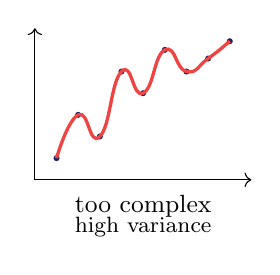
\begin{tikzpicture}[scale=0.55]
  \draw[->] (0,0) -- (5,0); \draw[->] (0,0) -- (0,3.5);
  \foreach \x/\y in {0.5/0.5, 1/1.5, 1.5/1.0, 2/2.5, 2.5/2.0, 3/3.0, 3.5/2.5, 4/2.8, 4.5/3.2} {
    \fill[darkblue] (\x,\y) circle (2pt);
  }
  \draw[softred, very thick, smooth, tension=0.9] plot coordinates {(0.5,0.5)(1,1.5)(1.5,1.0)(2,2.5)(2.5,2.0)(3,3.0)(3.5,2.5)(4,2.8)(4.5,3.2)};
  \node at (2.5, -0.6) {\small too complex};
  \node at (2.5, -1.1) {\footnotesize high variance};
\end{tikzpicture}
\end{columns}

\vspace{0.5em}
\centering
\textbf{Golden rule:} Never evaluate a model on the data used to train it!

Next lecture topic: Cross-Validation (Chapter 5) formalizes this
\end{frame}


\begin{frame}{Advertising: The Full Story}
\begin{columns}
\column{0.5\textwidth}
\textbf{Model comparison:}

\begin{tabular}{lc}
\toprule
Model & $R^2$ \\
\midrule
Sales $\sim$ TV & 0.612 \\
Sales $\sim$ TV + Radio & 0.897 \\
Sales $\sim$ TV + Radio + News & 0.897 \\
Sales $\sim$ TV $\times$ Radio & \textcolor{softgreen}{0.968} \\
\bottomrule
\end{tabular}

\vspace{0.3em}
Adding Radio: huge jump!

Adding Newspaper: nothing

Adding interaction: best model

\column{0.45\textwidth}
\textbf{Marketing recommendations:}

\begin{enumerate}
  \item Invest in \textbf{TV} and \textbf{Radio}
  \item Drop \textbf{Newspaper} budget
  \item Plan TV and Radio \textbf{jointly}\\
    (synergy effect!)
  \item Don't extrapolate beyond\\
    observed budget ranges
\end{enumerate}
\end{columns}
\end{frame}


\begin{frame}{Auto Data: Linear vs.\ Quadratic in Detail}
\begin{columns}
\column{0.48\textwidth}
\textbf{Linear:} mpg $\sim$ hp

\begin{tabular}{lr}
\toprule
Metric & Value \\
\midrule
$R^2$ & 0.606 \\
RSE & 4.91 \\
$\hat{\beta}_1$ & $-0.158$ \\
\bottomrule
\end{tabular}

\vspace{0.3em}
Residual plot: U-shape!

\column{0.48\textwidth}
\textbf{Quadratic:} mpg $\sim$ hp + hp$^2$

\begin{tabular}{lr}
\toprule
Metric & Value \\
\midrule
$R^2$ & \textcolor{softgreen}{0.688} \\
RSE & \textcolor{softgreen}{4.37} \\
$\hat{\beta}_2$ & $0.0004$ \\
\bottomrule
\end{tabular}

\vspace{0.3em}
Residual plot: much better!
\end{columns}

\vspace{0.5em}
\centering
\textbf{ANOVA:} $F = 51.4$, $p < 10^{-11}$ $\Rightarrow$ quadratic term highly significant

\texttt{anova(linear\_fit, quad\_fit)}
\end{frame}


\begin{frame}{What Goes Into predict() ?}

\begin{columns}
\column{0.5\textwidth}
\texttt{predict(fit, newdata, interval)}

\vspace{0.5em}
\begin{tabular}{ll}
\toprule
Argument & What \\
\midrule
\texttt{fit} & your \texttt{lm()} object \\
\texttt{newdata} & data.frame with $X$ \\
\texttt{interval} & ``confidence'' or \\
 & ``prediction'' \\
\bottomrule
\end{tabular}

\column{0.45\textwidth}
\textbf{Example:}

\vspace{0.3em}
\footnotesize
\texttt{new <- data.frame(hp = 98)}

\texttt{predict(fit, new,}

\texttt{\phantom{predict(}interval = "confidence")}

\vspace{0.3em}
\normalsize
Returns: \texttt{fit}, \texttt{lwr}, \texttt{upr}

\vspace{0.3em}
\begin{tabular}{lcc}
\toprule
& CI & PI \\
\midrule
fit & 24.47 & 24.47 \\
lwr & 23.97 & 14.81 \\
upr & 24.96 & 34.12 \\
\bottomrule
\end{tabular}
\end{columns}
\end{frame}


\begin{frame}{Assumptions Checklist: Before You Trust Results}

\begin{center}
\begin{tikzpicture}[scale=0.85]
  \node[draw, fill=softgreen!10, rounded corners, minimum width=8cm, minimum height=0.7cm] at (0, 3) {\small 1. Linearity? $\quad\Rightarrow\quad$ Residuals vs Fitted};
  \node[draw, fill=softgreen!10, rounded corners, minimum width=8cm, minimum height=0.7cm] at (0, 2) {\small 2. Independence? $\quad\Rightarrow\quad$ Residuals vs Time order};
  \node[draw, fill=softgreen!10, rounded corners, minimum width=8cm, minimum height=0.7cm] at (0, 1) {\small 3. Constant variance? $\quad\Rightarrow\quad$ Scale-Location plot};
  \node[draw, fill=softgreen!10, rounded corners, minimum width=8cm, minimum height=0.7cm] at (0, 0) {\small 4. Normality? $\quad\Rightarrow\quad$ Q-Q plot};
  \node[draw, fill=softgreen!10, rounded corners, minimum width=8cm, minimum height=0.7cm] at (0, -1) {\small 5. No multicollinearity? $\quad\Rightarrow\quad$ \texttt{car::vif(fit)}};
\end{tikzpicture}
\end{center}

\vspace{0.3em}
\centering
\textit{If assumptions are violated, inference (p-values, CIs) may be wrong!}
\end{frame}


\begin{frame}{Gauss-Markov: Why OLS Is Special}
\begin{columns}
\column{0.5\textwidth}
\textbf{Theorem:}

Among all \textbf{linear} and \textbf{unbiased} estimators of $\beta$,
OLS has the \textbf{smallest variance}.

\vspace{0.3em}
$\hat{\boldsymbol{\beta}}_{\text{OLS}}$ is \textbf{BLUE}:

\begin{itemize}
  \item \textbf{B}est
  \item \textbf{L}inear
  \item \textbf{U}nbiased
  \item \textbf{E}stimator
\end{itemize}

\column{0.45\textwidth}
\textbf{Requirements:}

\begin{enumerate}
  \item $E[\varepsilon_i] = 0$
  \item $\text{Var}(\varepsilon_i) = \sigma^2$
  \item $\text{Cov}(\varepsilon_i, \varepsilon_j) = 0$
\end{enumerate}

\vspace{0.5em}
\textbf{Note:}

\begin{itemize}
  \item Does NOT require normality!
  \item Normality needed only for\\exact $t$ and $F$ distributions
\end{itemize}
\end{columns}
\end{frame}


\begin{frame}{Beyond Week 1: The Road Ahead}

\begin{center}
\begin{tikzpicture}[scale=0.8, every node/.style={font=\small}]
  % Timeline
  \draw[thick, ->] (0,0) -- (12,0);

  \foreach \x/\lab/\col in {0.5/Linear Reg./accent, 2/Logistic/softgreen, 3.5/CV/amber, 5/Lasso/softgreen, 6.5/Splines/amber, 8/Trees/softgreen, 9.5/SVM/amber, 11/DL/softred} {
    \fill[\col] (\x, 0) circle (4pt);
    \node[above, rotate=45, anchor=south west] at (\x, 0.2) {\lab};
  }

  % Arrows showing connections
  \draw[->, thick, accent!50] (0.5, -0.5) to[bend right=30] node[below, font=\footnotesize] {\textit{all build on this}} (8, -0.5);
\end{tikzpicture}
\end{center}

\vspace{0.5em}
\textbf{Linear regression limitations we'll address:}
\begin{itemize}
  \item Non-linearity $\Rightarrow$ Splines, Trees, Neural Nets
  \item Too many predictors $\Rightarrow$ Lasso, Ridge
  \item Model evaluation $\Rightarrow$ Cross-Validation
  \item Classification $\Rightarrow$ Logistic Regression, SVM
\end{itemize}
\end{frame}


% ══════════════════════════════════════════════
% EXERCISES
% ══════════════════════════════════════════════

\begin{frame}{Exercise 1: Auto Dataset (ISLR 3.7 Q8)}

\textbf{Data:} \texttt{Auto} from ISLR2 \hfill $n = 392$, $p = 8$

\vspace{0.5em}
\begin{enumerate}
  \item Fit SLR: \texttt{lm(mpg \textasciitilde{} horsepower)}
  \item Interpret $\hat{\beta}_1$ in words
  \item Predict mpg at horsepower $= 98$
  \item Compute 95\% CI and PI at hp $= 98$
  \item Plot data with regression line
  \item Check diagnostic plots --- any problems?
\end{enumerate}

\vspace{0.5em}
\fbox{\textbf{Hint:} Expect $R^2 \approx 0.61$ and a U-shaped residual plot}
\end{frame}


\begin{frame}{Exercise 2: Multiple Regression (ISLR 3.7 Q9)}

\textbf{Data:} \texttt{Auto} \hfill Fit: \texttt{mpg \textasciitilde{} . - name}

\vspace{0.5em}
\begin{enumerate}
  \item Produce a scatterplot matrix
  \item Compute correlation matrix
  \item Fit MLR with all predictors
  \item Which predictors are significant?
  \item What does the \texttt{year} coefficient mean?
  \item Check residual plots
  \item Try interaction terms --- which are significant?
  \item Try $\log$, $\sqrt{X}$, $X^2$ --- do they improve fit?
\end{enumerate}
\end{frame}


\begin{frame}{Exercise 3: Carseats (ISLR 3.7 Q10)}

\textbf{Data:} \texttt{Carseats} \hfill $n = 400$

\vspace{0.5em}
Fit: \texttt{Sales \textasciitilde{} Price + Urban + US}
\begin{enumerate}
  \item Interpret each coefficient
  \item For which can you reject $H_0$?
  \item Fit reduced model (significant predictors only)
  \item Compare $R^2$, Adj.\ $R^2$, RSE
  \item 95\% CIs for the reduced model
\end{enumerate}

\vspace{0.5em}
\fbox{\textbf{Key finding:} Urban is not significant ($p \approx 0.94$)}
\end{frame}


\begin{frame}{Exercise 4: Boston EDA (ISLR 2.4 Q10)}

\textbf{Data:} \texttt{Boston} \hfill $n = 506$ census tracts

\vspace{0.5em}
\begin{enumerate}
  \item How many rows/columns?
  \item Pairwise scatterplots for selected variables
  \item Which predictors associate with crime rate?
  \item Tracts with extreme crime, tax, ptratio?
  \item How many tracts bound the Charles River?
  \item Median pupil-teacher ratio?
  \item Tract with lowest median home value --- comment
\end{enumerate}

\vspace{0.5em}
\fbox{\textbf{Hint:} \texttt{cor(Boston)[, "crim"]} reveals strongest associations}
\end{frame}


\begin{frame}{Solution: Exercise 1 --- Key Results}
\begin{columns}
\column{0.5\textwidth}
$\hat{\beta}_1 = -0.158$, $p < 10^{-16}$

\vspace{0.2em}
Each unit hp $\Rightarrow$ mpg drops by 0.16

\vspace{0.2em}
At hp $= 98$: $\hat{Y} = 24.47$

\vspace{0.2em}
95\% CI: $[23.97, \; 24.96]$

95\% PI: $[14.81, \; 34.12]$

\vspace{0.3em}
$R^2 = 0.606$, RSE $= 4.91$

\column{0.45\textwidth}
\textbf{Residual plot:}

\begin{tikzpicture}[scale=0.6]
  \draw[->, thick] (0,0) -- (5,0) node[right] {\small $\hat{y}$};
  \draw[->, thick] (0,-2) -- (0,2) node[above] {\small $e$};
  \draw[muted, dashed] (0,0) -- (5,0);
  \draw[softred, thick, smooth, tension=0.5] plot coordinates {(0.3,-0.5)(1.5,0.8)(2.5,0.3)(3.5,-0.5)(4.5,-0.8)};
  \node[softred] at (2.5, -2.3) {\footnotesize \textbf{U-shape!} Add hp$^2$};
\end{tikzpicture}

\vspace{0.2em}
With quadratic: $R^2 = 0.688$
\end{columns}
\end{frame}


\begin{frame}{Solution: Exercise 2 --- Key Results}
\begin{columns}
\column{0.55\textwidth}
\textbf{Significant predictors:}

displacement, weight, year, origin

\vspace{0.3em}
\textbf{Not significant:}

\textcolor{softred}{horsepower} (collinear with weight)

\vspace{0.3em}
\textbf{Year coefficient $\approx 0.75$:}

Each model year $\Rightarrow$ +0.75 mpg

(technology improves efficiency)

\column{0.4\textwidth}
\textbf{Improvements:}

\vspace{0.3em}
\begin{tabular}{lc}
\toprule
Model & $R^2$ \\
\midrule
All linear & 0.82 \\
+ interactions & 0.86 \\
+ $\log$ terms & 0.87 \\
\bottomrule
\end{tabular}

\vspace{0.3em}
\footnotesize displacement $\times$ weight\\interaction is significant
\end{columns}
\end{frame}


\begin{frame}{Solution: Exercise 3 --- Carseats}

\begin{columns}
\column{0.5\textwidth}
\begin{tabular}{lrl}
\toprule
 & $\hat{\beta}$ & $p$ \\
\midrule
Price & $-0.054$ & $< 0.001$ \\
Urban & $-0.022$ & \textcolor{softred}{0.936} \\
US & $+1.201$ & $< 0.001$ \\
\bottomrule
\end{tabular}

\vspace{0.5em}
\textbf{Reduced model:}

\texttt{Sales \textasciitilde{} Price + US}

\vspace{0.3em}
Adj.\ $R^2$ slightly improves!

\column{0.45\textwidth}
\textbf{Interpretation:}

\begin{itemize}
  \item \$1 more $\Rightarrow$ 0.054 fewer units sold
  \item Urban/Rural: no difference
  \item US stores sell 1.2 more units
\end{itemize}

\vspace{0.3em}
\textcolor{accent}{\textit{Drop Urban, keep Price + US}}
\end{columns}
\end{frame}


\begin{frame}{Solution: Exercise 4 --- Boston}
\begin{columns}
\column{0.5\textwidth}
\begin{itemize}
  \item $n = 506$, $p = 13$
  \item Crime correlates with:\\rad ($r=0.63$), tax ($r=0.58$)
  \item 35 tracts bound Charles River
  \item Median ptratio $= 19.05$
\end{itemize}

\column{0.45\textwidth}
\textbf{Lowest medv tract:}

\begin{tabular}{lr}
\toprule
Variable & Value \\
\midrule
crim & 38.35 \\
age & 100 \\
lstat & 30.59 \\
medv & \$5k \\
\bottomrule
\end{tabular}

\vspace{0.2em}
\footnotesize Most disadvantaged area
\end{columns}
\end{frame}


\begin{frame}{Conceptual Solutions (ISLR 2.4 Q1)}

\textbf{Flexible or inflexible method?}

\vspace{0.5em}
\begin{tabular}{llp{5cm}}
\toprule
Scenario & Best & Why \\
\midrule
(a) Large $n$, small $p$ & Flexible & Enough data to avoid overfit \\
(b) Small $n$, large $p$ & Inflexible & High overfit risk \\
(c) Non-linear $f$ & Flexible & Rigid model has high bias \\
(d) High $\text{Var}(\varepsilon)$ & Inflexible & Flexible follows noise \\
\bottomrule
\end{tabular}

\vspace{0.5em}
\centering
\textit{Always think: bias--variance trade-off!}
\end{frame}


\begin{frame}{Conceptual: Sketch the Curves (ISLR 2.4 Q3)}

\begin{center}
\begin{tikzpicture}[scale=0.75]
  \draw[->, thick] (0,0) -- (7,0) node[below] {\small Flexibility};
  \draw[->, thick] (0,0) -- (0,5) node[above] {\small Error/Value};

  % Squared Bias
  \draw[accent, very thick, domain=0.3:6.5, samples=50] plot (\x, {3.8*exp(-0.45*\x)});
  \node[accent, right] at (5.5, 0.4) {\small Bias$^2$};

  % Variance
  \draw[amber, very thick, domain=0.3:6.5, samples=50] plot (\x, {0.06*\x*\x});
  \node[amber, right] at (5.5, 2.6) {\small Variance};

  % Training MSE
  \draw[softgreen!70!black, thick, domain=0.3:6.5, samples=50] plot (\x, {3.5*exp(-0.5*\x) + 0.1});
  \node[softgreen!70!black, right] at (5.5, 0.2) {\small Train MSE};

  % Test MSE
  \draw[softred, very thick, domain=0.3:6.5, samples=50] plot (\x, {3.8*exp(-0.45*\x) + 0.06*\x*\x + 0.4});
  \node[softred, right] at (5.5, 3.2) {\small Test MSE};

  % Bayes error
  \draw[muted, dashed, thick] (0.3, 0.4) -- (6.8, 0.4);
  \node[muted, right] at (5.5, 0.55) {\small Bayes};
\end{tikzpicture}
\end{center}

5 curves: Bias$^2$ (decreasing), Variance (increasing), Test MSE (U-shape),\\
Training MSE (decreasing), Bayes error (constant horizontal line)
\end{frame}


\begin{frame}{Conceptual: Training RSS --- Linear vs.\ Cubic (ISLR 3.7 Q4)}

\begin{columns}
\column{0.48\textwidth}
\textbf{(a) True $f$ is linear:}

\vspace{0.3em}
Training RSS:

Cubic $\leq$ Linear

\vspace{0.3em}
\textit{More flexible always fits training data at least as well}

\vspace{0.5em}
\textbf{(b) Test RSS:}

Linear $\leq$ Cubic (probably)

\vspace{0.3em}
\textit{Cubic overfits --- estimates noise as signal}

\column{0.48\textwidth}
\textbf{(c) True $f$ is non-linear:}

\vspace{0.3em}
Training RSS:

Cubic $\leq$ Linear (always)

\vspace{0.5em}
\textbf{(d) Test RSS:}

\textit{Not enough information!}

\vspace{0.3em}
Depends on how far from linear:
\begin{itemize}
  \item Slightly non-linear: linear may win
  \item Very non-linear: cubic wins
\end{itemize}
\end{columns}
\end{frame}


\begin{frame}{Regression vs.\ Classification: Practice (ISLR 2.4 Q2)}
\begin{center}
\begin{tabular}{llccl}
\toprule
Scenario & Type & $n$ & $p$ & Goal \\
\midrule
(a) CEO salary & Regression & 500 & 3 & Inference \\
(b) Product launch & Classification & 20 & 13 & Prediction \\
(c) Exchange rate & Regression & 52 & 3 & Prediction \\
\bottomrule
\end{tabular}
\end{center}

\vspace{0.5em}
\textbf{Key distinctions:}
\begin{itemize}
  \item CEO salary is continuous $\Rightarrow$ regression + inference (``which factors?'')
  \item Success/failure is binary $\Rightarrow$ classification + prediction
  \item \% change is continuous $\Rightarrow$ regression + prediction
\end{itemize}
\end{frame}


\begin{frame}{The ``No Free Lunch'' Theorem --- Visually}

\begin{columns}
\column{0.48\textwidth}
\textbf{Dataset A:}

\begin{tikzpicture}[scale=0.55]
  \draw[->] (0,0) -- (4.5,0); \draw[->] (0,0) -- (0,3.5);
  \foreach \x/\y in {0.5/0.5, 1/1.0, 1.5/1.5, 2/2.0, 2.5/2.5, 3/3.0, 3.5/3.2} {
    \fill[darkblue] (\x,\y) circle (2pt);
  }
  \draw[softgreen, very thick] (0.3, 0.3) -- (3.7, 3.4);
  \node[softgreen] at (2, -0.5) {\footnotesize Linear wins!};
\end{tikzpicture}

\column{0.48\textwidth}
\textbf{Dataset B:}

\begin{tikzpicture}[scale=0.55]
  \draw[->] (0,0) -- (4.5,0); \draw[->] (0,0) -- (0,3.5);
  \foreach \x/\y in {0.5/0.5, 1/2.5, 1.5/1.0, 2/3.0, 2.5/0.8, 3/2.8, 3.5/1.5} {
    \fill[darkblue] (\x,\y) circle (2pt);
  }
  \draw[softred, thick, dashed] (0.3, 1.5) -- (3.7, 1.8);
  \draw[softgreen, very thick, smooth, tension=0.7] plot coordinates {(0.5,0.5)(1,2.5)(1.5,1.0)(2,3.0)(2.5,0.8)(3,2.8)(3.5,1.5)};
  \node[softgreen] at (2, -0.5) {\footnotesize KNN wins!};
\end{tikzpicture}
\end{columns}

\vspace{0.5em}
\centering
\fbox{\parbox{0.7\textwidth}{\centering
\textbf{No single method is best for all datasets.}\\
The best method depends on the data structure.}}
\end{frame}


\begin{frame}{Bias-Variance for KNN: $K$ Controls Everything}

\begin{center}
\begin{tikzpicture}[scale=0.8]
  \draw[->, thick] (0,0) -- (8,0) node[below] {\small $1/K$ (flexibility)};
  \draw[->, thick] (0,0) -- (0,5) node[above] {\small Error};

  % Training error
  \draw[accent, very thick, domain=0.5:7, samples=50] plot (\x, {3*exp(-0.6*\x) + 0.1});
  \node[accent, right] at (6.5, 0.3) {\small Train};

  % Test error
  \draw[softred, very thick, domain=0.5:7, samples=50] plot (\x, {0.08*(\x-3)^2 + 1.2});
  \node[softred, right] at (6.5, 2.4) {\small Test};

  % Labels
  \node[below] at (0.8, -0.3) {\small $K=100$};
  \node[below] at (6.5, -0.3) {\small $K=1$};
  \draw[softgreen, dashed] (3, 0) -- (3, 1.2);
  \fill[softgreen] (3, 1.2) circle (3pt);
  \node[softgreen, below] at (3, -0.3) {\small $K^*$};
\end{tikzpicture}
\end{center}

\begin{itemize}
  \item At $K=1$: Training error $= 0$, but test error is high (overfit)
  \item At $K=n$: Every prediction $= \bar{y}$ (underfit)
  \item Optimal $K^*$ minimizes test error
\end{itemize}
\end{frame}


\begin{frame}{How Many Predictors Is Too Many?}

\begin{columns}
\column{0.55\textwidth}
\textbf{Rule of thumb:}

Need $\approx 10$--$20$ observations per predictor

\vspace{0.3em}
\begin{tabular}{ccc}
\toprule
$n$ & $p$ & Ratio \\
\midrule
200 & 3 & 67 \textcolor{softgreen}{\checkmark} \\
100 & 10 & 10 \textcolor{amber}{$\sim$} \\
50 & 20 & 2.5 \textcolor{softred}{$\times$} \\
30 & 50 & 0.6 \textcolor{softred}{$\times\times$} \\
\bottomrule
\end{tabular}

\column{0.4\textwidth}
\textbf{When $p > n$:}

\begin{itemize}
  \item OLS doesn't work! ($\mathbf{X}^T\mathbf{X}$ singular)
  \item $R^2 = 1$ trivially
  \item Need regularization (Ch 6)
  \item Lasso / Ridge to the rescue
\end{itemize}
\end{columns}

\vspace{0.5em}
\centering
\textit{High dimensions: Chapter 6 will save you!}
\end{frame}


\begin{frame}{Residual Analysis: A 3-Step Workflow}

\begin{center}
\begin{tikzpicture}[scale=0.85, every node/.style={font=\small}]
  \node[draw, fill=accent!15, rounded corners, minimum width=3cm, minimum height=1cm] (s1) at (0,0) {\textbf{Step 1:} Fit model};
  \node[draw, fill=amber!15, rounded corners, minimum width=3cm, minimum height=1cm] (s2) at (5,0) {\textbf{Step 2:} Check plots};
  \node[draw, fill=softgreen!15, rounded corners, minimum width=3cm, minimum height=1cm] (s3) at (10,0) {\textbf{Step 3:} Fix issues};

  \draw[->, very thick] (s1) -- (s2);
  \draw[->, very thick] (s2) -- (s3);
  \draw[->, thick, muted, dashed] (s3) to[bend right=40] node[below, font=\footnotesize] {iterate} (s1);
\end{tikzpicture}
\end{center}

\vspace{0.5em}
\begin{columns}
\column{0.32\textwidth}
\centering
\texttt{fit <- lm(...)}

\texttt{summary(fit)}

\column{0.32\textwidth}
\centering
\texttt{plot(fit)}

\texttt{car::vif(fit)}

\column{0.32\textwidth}
\centering
Add $X^2$, $\log(Y)$

Remove collinear $X$
\end{columns}

\vspace{0.5em}
\centering
\textit{Regression is iterative, not one-shot!}
\end{frame}


\begin{frame}{Comparing Nested Models: The ANOVA Approach}

\textbf{Model 1:} mpg $\sim$ horsepower \hfill (reduced)

\textbf{Model 2:} mpg $\sim$ horsepower + horsepower$^2$ \hfill (full)

\vspace{0.5em}
$$F = \frac{(\text{RSS}_1 - \text{RSS}_2) / (\text{df}_1 - \text{df}_2)}{\text{RSS}_2 / \text{df}_2}$$

\vspace{0.5em}
\begin{columns}
\column{0.5\textwidth}
\textbf{Numbers:}

$\text{RSS}_1 = 9386$, $\text{df}_1 = 390$

$\text{RSS}_2 = 7442$, $\text{df}_2 = 389$

$$F = \frac{(9386-7442)/1}{7442/389} = 101.6$$

\column{0.45\textwidth}
$p$-value $< 10^{-11}$

\vspace{0.3em}
\textcolor{softgreen}{\textbf{Quadratic term is highly significant}}

\vspace{0.5em}
\footnotesize R: \texttt{anova(fit1, fit2)}

Tests whether the extra predictor(s)\\
provide a significant improvement
\end{columns}
\end{frame}


\begin{frame}{Quick Quiz: Test Yourself!}

\begin{enumerate}
  \item What does $R^2 = 0.75$ mean?
  \pause
  \item[]{\textcolor{muted}{\footnotesize 75\% of variance in $Y$ is explained by the model}}

  \vspace{0.3em}
  \item A coefficient has $p = 0.03$. Is it significant at $\alpha = 0.05$?
  \pause
  \item[]{\textcolor{muted}{\footnotesize Yes --- $0.03 < 0.05$, reject $H_0$}}

  \vspace{0.3em}
  \item VIF$_j = 12$. What does this mean?
  \pause
  \item[]{\textcolor{muted}{\footnotesize Severe collinearity --- $X_j$ is almost a linear combination of other predictors}}

  \vspace{0.3em}
  \item Prediction interval is always wider than confidence interval. Why?
  \pause
  \item[]{\textcolor{muted}{\footnotesize PI includes $\text{Var}(\varepsilon)$ on top of coefficient uncertainty}}
\end{enumerate}
\end{frame}


\begin{frame}{Quick Quiz: More Questions}

\begin{enumerate}
  \setcounter{enumi}{4}
  \item Residual plot shows U-shape. What's wrong?
  \pause
  \item[]{\textcolor{muted}{\footnotesize Non-linearity --- add polynomial or transformation}}

  \vspace{0.3em}
  \item Can $R^2$ decrease when you add a predictor?
  \pause
  \item[]{\textcolor{muted}{\footnotesize $R^2$: never. Adjusted $R^2$: yes, if the predictor is useless}}

  \vspace{0.3em}
  \item $\hat{\beta}_1 = -0.05$, $\text{SE} = 0.08$. Is this significant?
  \pause
  \item[]{\textcolor{muted}{\footnotesize $t = -0.05/0.08 = -0.625$. No --- $|t| < 2$, $p$ is large}}

  \vspace{0.3em}
  \item When does KNN beat linear regression?
  \pause
  \item[]{\textcolor{muted}{\footnotesize When $f$ is highly non-linear AND $p$ is small}}
\end{enumerate}
\end{frame}


\begin{frame}{The Advertising Correlation Matrix}

\begin{columns}
\column{0.5\textwidth}
\begin{tabular}{lcccc}
\toprule
 & TV & Radio & News & Sales \\
\midrule
TV & 1.00 & 0.05 & 0.06 & \textcolor{softgreen}{\textbf{0.78}} \\
Radio & 0.05 & 1.00 & \textcolor{amber}{0.35} & \textcolor{softgreen}{\textbf{0.58}} \\
News & 0.06 & \textcolor{amber}{0.35} & 1.00 & 0.23 \\
Sales & \textcolor{softgreen}{\textbf{0.78}} & \textcolor{softgreen}{\textbf{0.58}} & 0.23 & 1.00 \\
\bottomrule
\end{tabular}

\column{0.45\textwidth}
\textbf{Key observations:}

\begin{itemize}
  \item TV strongest predictor
  \item Radio--News: $r = 0.35$\\
    This is the confounder!
  \item TV \& Radio are nearly\\
    uncorrelated ($r = 0.05$)
\end{itemize}
\end{columns}

\vspace{0.5em}
\centering
\footnotesize R: \texttt{round(cor(Advertising[, -5]), 2)}
\end{frame}


\begin{frame}{Key Takeaway: The Regression Workflow}

\begin{center}
\begin{tikzpicture}[scale=0.75, every node/.style={font=\small, text width=2.5cm, align=center}]
  \node[draw, fill=accent!15, rounded corners, minimum height=1cm] (q) at (0,3) {Ask a\\question};
  \node[draw, fill=accent!15, rounded corners, minimum height=1cm] (eda) at (3.5,3) {Explore\\data (EDA)};
  \node[draw, fill=accent!15, rounded corners, minimum height=1cm] (fit) at (7,3) {Fit\\model};
  \node[draw, fill=amber!15, rounded corners, minimum height=1cm] (check) at (7,0.5) {Check\\assumptions};
  \node[draw, fill=amber!15, rounded corners, minimum height=1cm] (fix) at (3.5,0.5) {Revise\\model};
  \node[draw, fill=softgreen!15, rounded corners, minimum height=1cm] (report) at (0,0.5) {Report\\results};

  \draw[->, very thick] (q) -- (eda);
  \draw[->, very thick] (eda) -- (fit);
  \draw[->, very thick] (fit) -- (check);
  \draw[->, very thick] (check) -- (fix);
  \draw[->, very thick, muted] (fix) -- (fit);
  \draw[->, very thick] (fix) -- (report);
\end{tikzpicture}
\end{center}

\vspace{0.3em}
\centering
\textit{Regression is a conversation with data, not a single command.}
\end{frame}


\begin{frame}{What's Next?}

\begin{center}
\begin{tikzpicture}[scale=0.8]
  \node[draw, fill=accent!30, rounded corners, minimum width=3.5cm, minimum height=0.8cm, font=\bfseries] (w1) at (0,0) {Week 1: Linear Reg.};
  \node[draw, fill=softgreen!20, rounded corners, minimum width=3.5cm, minimum height=0.8cm] (w2) at (0,-1.5) {Week 2: Classification};
  \node[draw, fill=softgreen!20, rounded corners, minimum width=3.5cm, minimum height=0.8cm] (w3) at (0,-3.0) {Week 3: Cross-Validation};
  \node[draw, fill=softgreen!20, rounded corners, minimum width=3.5cm, minimum height=0.8cm] (w4) at (0,-4.5) {Week 4: Lasso \& Ridge};
  \draw[->, thick] (w1) -- (w2);
  \draw[->, thick] (w2) -- (w3);
  \draw[->, thick] (w3) -- (w4);
\end{tikzpicture}
\end{center}

\vspace{0.3em}
\textbf{Homework:} ISLR Chapter 2: Q1, 2, 3, 10 \quad|\quad Chapter 3: Q8, 9, 10

\textbf{Lab:} \texttt{Lab\_Week1.R} from \texttt{github.com/endri81/ISLRv2-solutions}
\end{frame}


\begin{frame}{}
\centering
\vspace{2cm}
{\Huge\textbf{Thank You}}

\vspace{1em}
{\Large Questions?}

\vspace{1.5em}
{\large Dr.\ Endri Ra\c{c}o \quad|\quad Machine Learning with R}

\vspace{0.5em}
{\normalsize \texttt{github.com/endri81/ISLRv2-solutions}}
\end{frame}

\end{document}
